\documentclass[twoside]{article}

% Fonts + Colors ~~~~

\usepackage{lipsum}
\usepackage{fontspec}
\usepackage{dashrule}
\usepackage[export]{adjustbox}
\usepackage[usenames, dvipsnames]{color}
\usepackage{comment}

\definecolor{Gray}{RGB}{120, 120, 120}
\definecolor{LogoRed}{RGB}{153, 0, 0}
\definecolor{LogoTurquoise1}{RGB}{1, 123, 147}
\definecolor{LogoTurquoise2}{RGB}{0, 158, 171}
\definecolor{LogoTurquoise3}{RGB}{0, 186, 187}
\definecolor{BackgroundBlue}{RGB}{247, 254, 255}
\definecolor{LightBlue}{RGB}{230, 247, 255}
\definecolor{LightRed}{RGB}{231, 103, 97}
\definecolor{DarkGray}{RGB}{71, 71, 71}

\begin{comment}
\newfontfamily\Avenir[
    Path= fonts/,
    Extension= .otf,
    UprightFont = *-45Book,
    ItalicFont = *-45BookOblique,
    BoldFont = *-95Black,
]{AvenirLTStd}

\newfontfamily\TradeGothic[
    Path = fonts/,
    Extension = .otf,
    UprightFont = *-No18,
    BoldFont = *-No20Bold,
]{TradeGothicCondensed}

\setmainfont[Ligatures=TeX]{Avenir}
\Avenir\fontsize{9pt}{12pt}\selectfont

\end{comment}

\usepackage[condensed]{roboto}
\usepackage[default,osfigures,scale=0.95]{opensans}
\usepackage[T1]{fontenc}

\fontsize{9pt}{12pt}\selectfont

% Formatting ~~~~

\usepackage{geometry}

\geometry{
    letterpaper,
    top=1.75in,
    bottom=1.75in,
    inner=0.75in,
    outer=0.75in,
    headsep=1in,
    headheight=0.5in,
    footskip=1in,
    % showframe
}

\usepackage[document]{ragged2e}
\parskip=8pt
\parindent=0pt
\linespread{1.2}
\setlength{\columnsep}{0.75cm}

% \usepackage{sectsty}
% \sectionfont{\fontfamily{pag}\selectfont\color{LogoTurquoise1}\vspace{-\parskip}\Large\uppercase}
% \subsectionfont{\color{LogoTurquoise1}\vspace{-\parskip}\mdseries\Large}

\usepackage{titlesec}
\titleformat*{\section}{\fontfamily{pag}\selectfont\color{LogoTurquoise1}\vspace{-\parskip}\bfseries\Large\uppercase}
\titleformat*{\subsection}{\color{LogoTurquoise1}\vspace{-\parskip}\Large}


% Headers + Footers ~~~~

\usepackage{fancyhdr}
\pagestyle{fancy}

\renewcommand{\sectionmark}[1]{\markboth{#1}{}}
\usepackage{fourier-orns}

\fancyhead{} % clear all header fields
\fancyfoot{} % clear all footer fields
\fancyfoot[LE]{\thepage \hspace{0.4cm} \roboto\selectfont\textcolor{LightRed}{\uppercase{Recruiting the Out-of-State University}}}
\fancyfoot[RO]{\roboto\selectfont\textcolor{Gray}{\leftmark} \hspace{0.4cm} \thepage}
\renewcommand{\headrulewidth}{0pt}

\fancypagestyle{tablepage}{  % No Header, Regular Footer
    \fancyhead{}
    \fancyfoot{}
    \renewcommand\headrule{\hrulefill
\raisebox{-2.1pt}[10pt][10pt]{\quad\decofourleft\decotwo\decofourright\quad}\hrulefill}
}

\addtolength{\skip\footins}{10pt}


% Links + Lists ~~~~

\PassOptionsToPackage{hyphens}{url}\usepackage[colorlinks=true, linkcolor=cyan, urlcolor=blue, citecolor=blue, breaklinks=true]{hyperref}
\newcommand{\superscript}[1]{$^{#1}$}

%reference list stuff
\usepackage[natbibapa]{apacite}

%\usepackage[super,numbers]{natbib}

\makeatletter
\renewcommand\@biblabel[1]{\superscript{#1}}
\makeatother

\renewcommand{\refname}{\vspace{-0.65cm}}

\usepackage{enumitem}
\setlist{nosep, itemsep=0pt, parsep=0pt}

\renewcommand{\labelitemi}{\color{LightRed}$\triangleright$}
\renewcommand{\labelitemii}{\color{LogoTurquoise2}$\cdot$}
\renewcommand\labelitemiii{$\circ$}


% Block Formats ~~~~

\usepackage{mdframed}

\newenvironment{quote-block}{  % quote block
    \begin{quote}
    \roboto\selectfont
    \color{LogoTurquoise2}
}
{
    \end{quote}
}

\newenvironment{color-block}[1][Key Points]{  % text block
    \vspace{0.5cm}
    \begin{mdframed}[backgroundcolor=LightBlue, linecolor=LightBlue, userdefinedwidth=\textwidth, leftmargin=0cm, innerleftmargin=1cm, innerrightmargin=2cm, innertopmargin=0.5cm, innerbottommargin=1cm]
    \color{DarkGray}
    \subsection*{\color{LogoTurquoise1}{\Large#1}}
    \vspace{-0.2cm}
}
{
    \end{mdframed}
    \vspace{0.2cm}
}


% Figures ~~~~

\usepackage{graphicx}
\usepackage{caption}
\usepackage[labelformat=simple]{subcaption}

\DeclareCaptionSubType*{figure}
\renewcommand\thesubfigure{}

\DeclareCaptionFont{CaptionFont}{\roboto\selectfont}
\DeclareCaptionFont{LightRed}{\color{LightRed}}

\captionsetup{labelfont={CaptionFont, LightRed}, figurename=FIGURE, tablename=TABLE}

\newcommand{\addFigure}[4][0.2] {  % Add single figure
\begin{figure}[!ht]
    \vspace{0.45cm}
    \centering

    \includegraphics[width=0.45\textwidth, trim={0 0 0 #1cm}, clip]{images/#2}
    \caption{\roboto\selectfont\textcolor{Gray}{\uppercase{#3}}}
    \label{fig:#4}

\end{figure}
}

\usepackage{stfloats}
\newcommand{\addFigureSet}[4] {  % Add 2x2 figure set
\begin{figure*}[#4]
    \vspace{0.45cm}
    \centering

    \begin{subfigure}[b]{.45\linewidth}
      \includegraphics[width=\linewidth, cfbox=Gray 0.4pt]{images/maps/#1_1}
      \caption{1}
    \end{subfigure}\hfill
    \begin{subfigure}[b]{.45\linewidth}
      \includegraphics[width=\linewidth, cfbox=Gray 0.4pt]{images/maps/#1_2}
      \caption{2}
    \end{subfigure}

    \smallskip

    \begin{subfigure}[b]{.45\linewidth}
      \includegraphics[width=\linewidth, cfbox=Gray 0.4pt]{images/maps/#1_3}
      \caption{3}
    \end{subfigure}\hfill
    \begin{subfigure}[b]{.45\linewidth}
      \includegraphics[width=\linewidth, cfbox=Gray 0.4pt]{images/maps/#1_4}
      \caption{4}
    \end{subfigure}

    \caption{\roboto\selectfont\textcolor{Gray}{\uppercase{#2}}}
    \label{fig:#3}

    \ifnum\pdfstrcmp{#4}{b}=0
      \vspace{-1cm}
    \else
      \vspace{0.45cm}
    \fi

\end{figure*}
}

\newcommand{\addSmallMultiples}[3] {  % Add 3x5 figure set
\begin{figure*}[t]
    \vspace{0.45cm}
    \centering

    \includegraphics[width=0.3\textwidth, cfbox=Gray 0.4pt, trim={0 1cm 0 0}, clip]{graphs/199193/#1}\hfill
    \includegraphics[width=0.3\textwidth, cfbox=Gray 0.4pt, trim={0 1cm 0 0}, clip]{graphs/186380/#1}\hfill
    \includegraphics[width=0.3\textwidth, cfbox=Gray 0.4pt, trim={0 1cm 0 0}, clip]{graphs/196097/#1}

    \smallskip

    \includegraphics[width=0.3\textwidth, cfbox=Gray 0.4pt, trim={0 1cm 0 0}, clip]{graphs/100751/#1}\hfill
    \includegraphics[width=0.3\textwidth, cfbox=Gray 0.4pt, trim={0 1cm 0 0}, clip]{graphs/106397/#1}\hfill
    \includegraphics[width=0.3\textwidth, cfbox=Gray 0.4pt, trim={0 1cm 0 0}, clip]{graphs/110635/#1}

    \smallskip

    \includegraphics[width=0.3\textwidth, cfbox=Gray 0.4pt, trim={0 1cm 0 0}, clip]{graphs/110653/#1}\hfill
    \includegraphics[width=0.3\textwidth, cfbox=Gray 0.4pt, trim={0 1cm 0 0}, clip]{graphs/201885/#1}\hfill
    \includegraphics[width=0.3\textwidth, cfbox=Gray 0.4pt, trim={0 1cm 0 0}, clip]{graphs/126614/#1}

    \smallskip

    \includegraphics[width=0.3\textwidth, cfbox=Gray 0.4pt, trim={0 1cm 0 0}, clip]{graphs/139959/#1}\hfill
    \includegraphics[width=0.3\textwidth, cfbox=Gray 0.4pt, trim={0 1cm 0 0}, clip]{graphs/155317/#1}\hfill
    \includegraphics[width=0.3\textwidth, cfbox=Gray 0.4pt, trim={0 1cm 0 0}, clip]{graphs/166629/#1}

    \smallskip

    \includegraphics[width=0.3\textwidth, cfbox=Gray 0.4pt, trim={0 1cm 0 0}, clip]{graphs/181464/#1}\hfill
    \includegraphics[width=0.3\textwidth, cfbox=Gray 0.4pt, trim={0 1cm 0 0}, clip]{graphs/215293/#1}\hfill
    \includegraphics[width=0.3\textwidth, cfbox=Gray 0.4pt, trim={0 1cm 0 0}, clip]{graphs/218663/#1}

    \caption{\roboto\selectfont\textcolor{Gray}{\uppercase{#2}}}
    \label{fig:#3}
\end{figure*}
}


% Tables ~~~~

\usepackage[figuresright]{rotating}
\usepackage{multirow}
\usepackage[table]{xcolor}

\usepackage{etoolbox}
\AfterEndEnvironment{table-env}{\restoregeometry\twocolumn}

\newenvironment{table-env}[3][10]{
  \clearpage
  \newgeometry{top=0.5in, bottom=1in, inner=0.75in, outer=0.75in, footskip=0.25in}
  \begin{sidewaystable}
  \fontsize{8pt}{#1pt}\selectfont
  \ifnum\pdfstrcmp{#2}{x}=-1
    \rotatebox[origin=c]{270}{\begin{minipage}{\textwidth}\caption{\roboto\selectfont\textcolor{Gray}{\uppercase{#2}}}\label{tbl:#3}\end{minipage}}
  \fi
}
{
  \end{sidewaystable}
  \clearpage
}

\newcommand{\addTable}[4][p] {  % Add Table

\begin{table*}[!hb]

    \ifnum\pdfstrcmp{#1}{l}=0
      \begin{sideways}
    \fi

    \centering

    \begingroup
      \fontsize{8pt}{10pt}\selectfont
      \input{tables/#2.tex}
    \endgroup

    \ifnum\pdfstrcmp{#1}{l}=0
      \end{sideways}
    \fi

    \vspace{0.2cm}
    \caption{\roboto\selectfont\textcolor{Gray}{\uppercase{#3}}}
    \label{tbl:#4}

    \vspace{-1cm}

\end{table*}

}


\usepackage{Sweave}
\begin{document}
\sloppy

\Sconcordance{concordance:joyce_report.tex:joyce_report.Rnw:%
1 4 1 1 0 4 1 1 18 486 1}



% Title Page ~~~~

\pagecolor{BackgroundBlue}
\newgeometry{top=0cm, bottom=0cm, left=0cm, right=0cm}
\begin{titlepage}

        \makebox[0pt][l]{%
          \raisebox{-0.49\totalheight}[0pt][0pt]{%
          \scalebox{-1}[1]{
            
\includegraphics[width=9in]{./images/layer.png}}}}%

        \hspace{-0.7cm}
        \makebox[0pt][l]{%
          \raisebox{-1.43\totalheight}[0pt][0pt]{%
            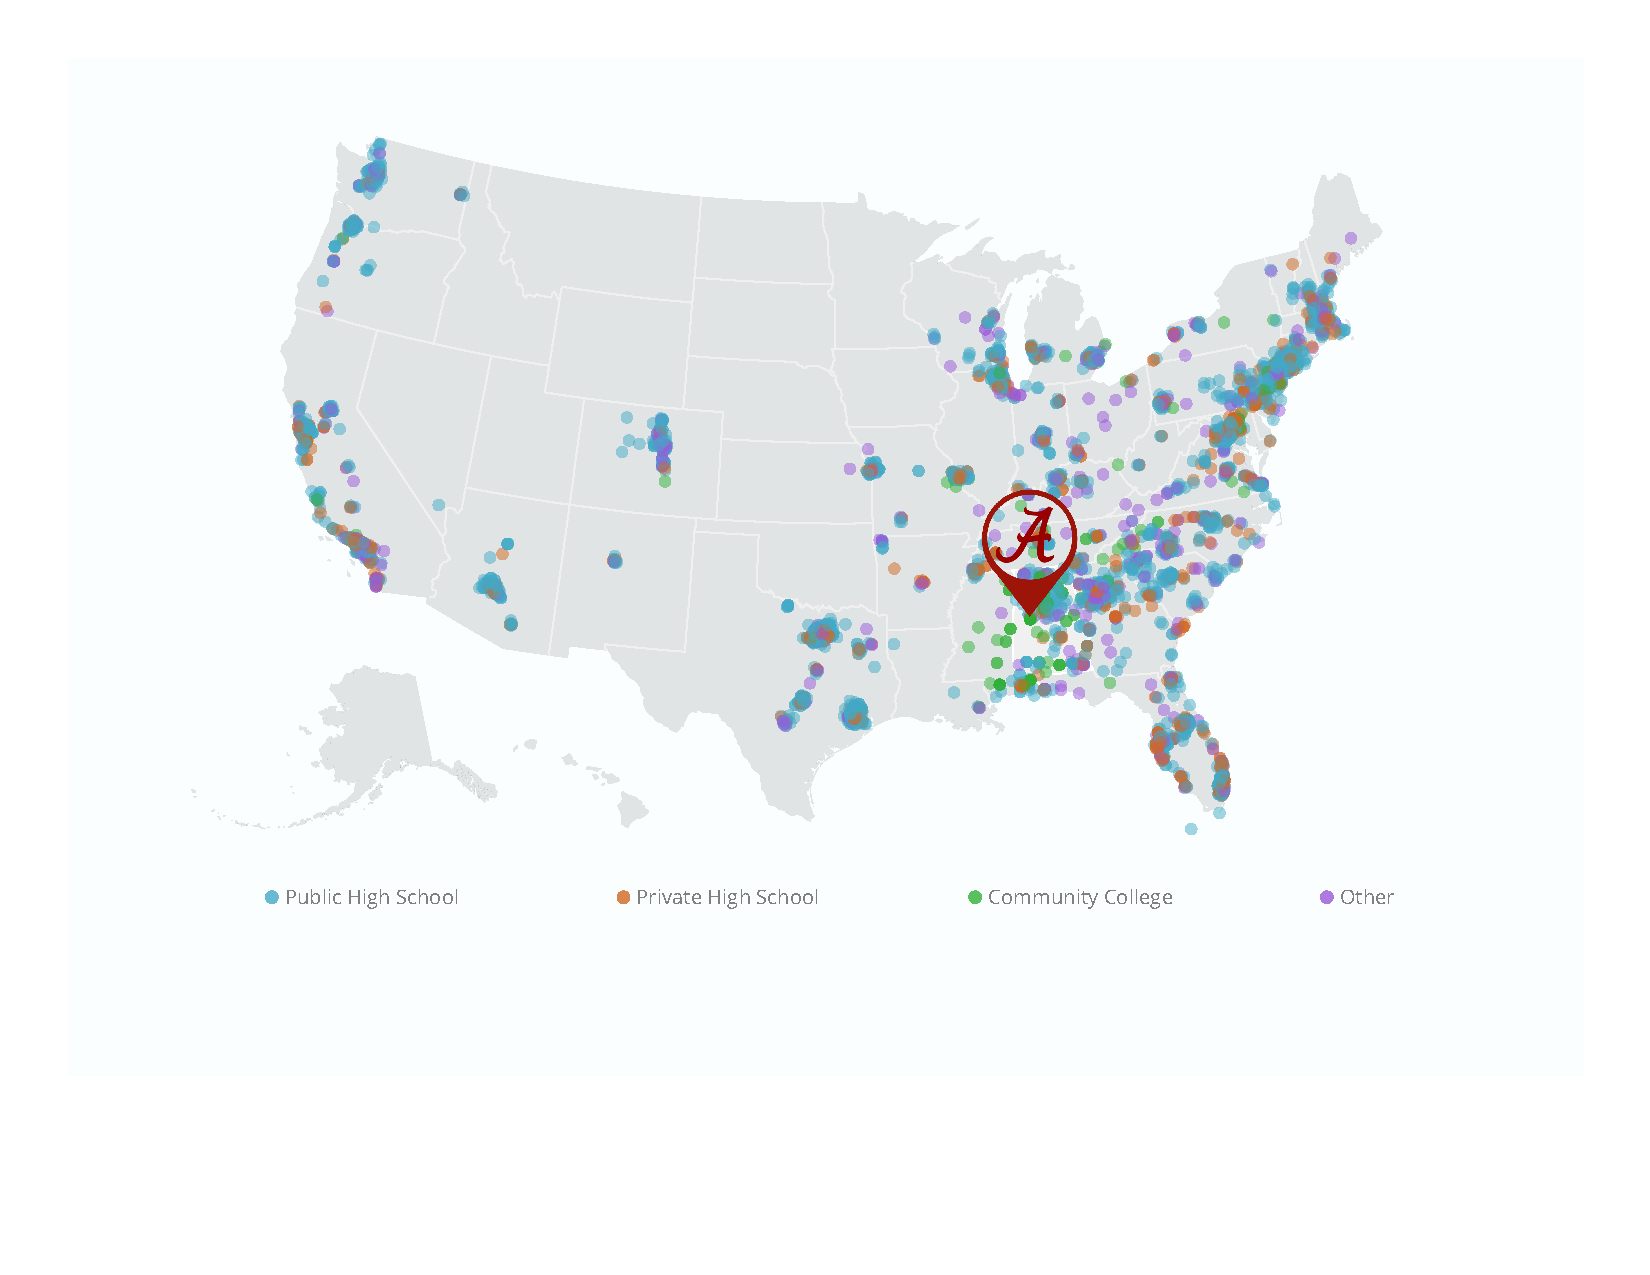
\includegraphics[width=9in, trim={2cm 0 2cm 2cm}, clip]{./images/map_ua.pdf}}}%

        \makebox[0pt][l]{%
          \raisebox{-1.44\totalheight}[0pt][0pt]{%
            
\includegraphics[width=9in]{./images/layer.png}}}%

        \centering\color{DarkGray}\fontsize{30}{60}

        \vspace{0.3cm}
        \hdashrule{0.8\textwidth}{1pt}{1pt} \\

        \vspace{0.8cm}
        \textbf{\color{LogoRed}{RECRUITING}} \\
        \vspace{0.2cm}
        \textbf{\color{LogoRed}{THE OUT-OF-STATE UNIVERSITY}}

        \vspace{0.2cm}
        \Large\textit{\fontfamily{pag}\selectfont Off-campus recruiting by public research universities} \\

        \vspace{0.3cm}
        \hdashrule{0.8\textwidth}{1pt}{1pt} \\

	\vspace{17.1cm}
        \large Crystal Han \\
        Ozan Jaquette \\
        Karina Salazar \\~\\
        %\textit{\color{Gray}{March 2019}}

\end{titlepage}

% Blank Page ~~~~
 
\pagecolor{LightBlue}
\begin{titlepage}
    \color{LightBlue}{x}
\end{titlepage}

% Begin Template ~~~~

\pagecolor{white}
\newgeometry{
    top=1.75in,
    bottom=1.25in,
    inner=1in,
    outer=1in,
    headsep=1in,
    headheight=0.5in,
    footskip=0.5in
}

\setcounter{page}{1}
\parskip=14pt
\linespread{1.3}

\section*{Executive Summary\markboth{Executive Summary}{}}  % text inside \markboth{} is displayed in footer

Despite a historical mission of social mobility for meritorious state residents, public research universities increasingly enroll an affluent student body that is unrepresentative of the socioeconomic and racial diversity of the states they serve.  Mainstream policy debates about the causes of access inequality focus on ``deficiencies'' of students and K-12 schools (e.g., the ``achievement gap,'' ``under-matching'').  Public universities positions themselves as remaining committed to access despite state funding cuts and despite student deficiencies, pointing to the adoption of access-oriented policies (e.g., need-based financial aid, outreach programs) as evidence of this commitment. Therefore, this discourse assumes that doubling the number of high-achieving, under-represented students who apply to a university will double their enrollment.  In turn, policy interventions to increase college access focus on changing student behavior rather than university behavior.

An alternative explanation for access inequality is that the enrollment priorities of some public research universities are biased against poor students and/or communities of color. Decades of research on organizational behavior finds that internal resource allocation is a reliable indicator of organizational priorities, while policy adoption is often a ceremonial effort to appease external stakeholders, suggesting a ``trust but verify'' approach to university rhetoric about access.  Scholarship on ``enrollment management'' shows that universities are very purposeful about which students they pursue and expend substantial resources crafting their class.  Therefore, knowing which student populations are targeted by university recruiting efforts can yield reliable insights about university enrollment priorities.

%Decades of research on organizational behavior finds that policy adoption is often a ceremonial effort to appease external stakeholders, while internal resource allocation provides a reliable indicator of organizational priorities. These findings suggest a ``trust but verify'' approach to university rhetoric about access
%often represents a ceremonial effort to appease external stakeholders rather than a substantive effort to solve the problem

This report analyzes off-campus recruiting visits (e.g., visit to a local high school) by 15 public research universities as a means of gaining insight about university enrollment priorities. We collected data on recruiting visits by “scraping” data from university admissions websites (e.g., webpages advertising admissions representatives coming to a ``neighborhood near you'') and by issuing public records requests. 
%Most universities exhibit systematic socioeconomic and racial inequities in off-campus recruiting patterns, but a small number of universities exhibit recruiting patterns broadly consistent with the historical mission of social mobility for meritorious state residents.
%We find that most universities exhibit systematic socioeconomic and racial inequities in off-campus recruiting patterns, 
%We find a startling degree of socioeconomic and racial bias in university off-campus recruiting patterns.

\begin{color-block}[Findings]

\textbf{Out-of-state recruiting visits}
\begin{itemize}
    \item \textbf{Most public research universities prioritize recruiting out-of-state students rather than students from their home state}. X of 15 universities made more out-of-state visits than in-state visits and X of 15 universities made more than twice as many out-of-state visits than in-state visits.
    \item Out-of-state visits in are concentrated in highly affluent communities in major metropolitan areas, ignoring rural communities
    \item All universities were much more likely to visit out-of-state public high schools in high-income communities than schools in low-income communities, even after controlling for other factors such as enrollment size and student achievement
    \item Most universities were significantly less likely to out-of-state visit public high schools with a high percentage of Black, Latinx, and Native American students, even after controlling for other factors
    \item Most universities visit a disproportionate number of out-of-state private schools
\end{itemize}

\textbf{In-state recruiting}
\begin{itemize}
    \item "Coverage" of in-state public high schools and community colleges varied dramatically across universities, even after considering state size and populatiion (e.g., University of Nebraska visited X\% of high schools while University of Alabama visited X\%)
    \item Most universities were more likely to visit in-state public high schools in high-income communities than schools in low income communities, even after controlling for other factors. However, income bias for in-state visits was smaller than income bias for out-of-state visits.
    \item The presence of racial bias in in-state visits to public high schools varied across universities, with some universities less likely to visit schools with a high share of Black/Latinx/Native students and other universities were more likely to visit schools with a high share of Black/Latinx/Native students
\end{itemize}  

\textbf{Overall patterns}
\begin{itemize}
    \item \textbf{Recruiting patterns are clearly tied to state funding}. Universities with weak state funding (e.g., University of Alabama, University of South Carolina) tended to make more out-of-state visits, fewer in-state visits, and exhibit socioeconomic and/or racial bias in in-state visits. %Universities with strong state funding (e.g., North Carolina State University, University of California-Irvine) tended make fewer out-of-state visits, more in-state visits, and exhibit less socioeconomic and/or racial bias in in-state visits
    \item Universities facing similar state funding and democgraphic trends (e.g., UC-Berkeley and UC-Irvine) often exhibited substantially different recruiting patterns with respect to out-of-state focus, income bias, and racial bias. Therefore, \textbf{university enrollment priorities are choices made by leadership rather than mere functions of environmental conditions.} 
    %\item Most universities followed the pattern of limited in-state recruiting and expansive out-of-state recruiting in large metropolitan areas, but the ``regional'' (e.g., Northeast, Midwest, Southeast) focus of out-of-state recruiting differed across universities    
\end{itemize}  

\end{color-block}

\textbf{Summary and implications}. In contrast to rhetoric from university leaders, our findings suggest strong socioeconomic and racial biases in the enrollment priorities of many public research universities. A small number of universities exhibit recruiting patterns broadly consistent with the historical mission of social mobility for meritorious state residents. However, most universities concentrated recruiting visits in wealthy, out-of-state communities. In-state visits also tended to privilege affluent schools. While most universities did not exhibit racial bias in in-state visits, out-of-state visits consistently exhibited racial bias.  Therefoe, the overall patterns of off-campus recruiting for most universities contribute to a student composition where low-income students of color feel increasingly isolated amongst growing cohorts of affluent, predominantly White, out-of-state students.

The recruiting patterns we observe a function of university enrollment priorities. In turn, these enrollment priorities are a function of a broken system of state higher education finance, which incentivizes many universities to prioritize rich out-of-state students with lack-luster academic achievement. This is not a meritocracy.  We suggest recommendations to policymakers, university leaders, and access advocates to reverse this vicious cycle.

	\begin{itemize}
		\item \textbf{State policymakers}. Universities make up for state budget cuts by prioritizing affluent students.  Therefore, if state policymakers want flagship public universities to prioritize meritorious state residents, they must re-invest in public higher education by growing state appropriations and/or by boosting the purchasing power of poor students through growth in need-based grant aid.
    \item \textbf{Access advocates}.  Advocates for access can use our research to start a dialogue with university leaders about the disconnect between stated commitments and actual enrollment priorities. Armed with systematic data about university recruiting behavior, access advocates will no longer be deterred by lofty rhetoric or the adoption of opaque programs with unclear resources. Therefore, the data and findings from this report enable access advocates to hold universities accountable, creating a foundation for an authentic debate about univeristy priorities.
		\item \textbf{University leaders}.  Research shows that generous need-based financial aid combined with aggressive outreach dramatically increases the number of high-achieving, low-income students who apply to and attend public research universities. Therefore, access inequality is not a simply a consequence of student deficiencies, but rather a deficit of will by universities.  University leaders serious about access for under-represented students must put their money where there mouth is, rather than putting their money where the money is.

	\end{itemize}

\newpage
\restoregeometry
\twocolumn

\section*{Introduction\markboth{Introduction}{}}  % text inside \markboth{} is displayed in footer

The University of Alabama-Tuscaloosa exemplifies that transformation from state flagship university to out-of-state flagship.  Resident freshmen increased from 2,028 in 2002-03 to 3,221 in 2008-09 but declined to 2,412 by 2016-17. By contrast, nonresident freshmen increased dramatically from 626 in 2002-03 to 1,895 in 2008-09 and to 5,147 by 2016-17.  This period was also witnessed the erosion of state appropriations, which had increased from  \$165 million in 2002-03 to \$227 million in 2007-08, but declined sharply to \$149 million by 2010-11 following the Great Recession, increasing only modestly to \$153 million by 2015-16 (2018 CPI).  By contrast, driving by nonresident enrollment growth, net tuition revenue increased dramatically, from \$102 million in 2002-03 to \$220 million by 2007-08 to \$492 million by 2015-16 [UPDATE NUMBERS/YEARS].

Nonresident enrollment growth at the University of Alabama also coincided with declining socioeconomic and racial diversity.  The percent of full-time freshman receiving Pell Grants declined from 21.2\% in 2010-11 to 17.1\% in 2016-17.  Additionally, while the percent of 18-24 year-olds in Alabama who identify as Black increased from 31.4\% in 2010-11 to 32.7\% in 2016-17 [GET NEW YEAR OF DATA?], the percent of full-time freshman at the University of Alabama who identify as Black declined from 11.9\%  in 2010-11 to 7.5\% in 2017-18.

While most research on college access focuses on student behavior, the transformation of student composition at the University of Alabama did not result from sudden, unexpected shifts in student demand. Rather, the University developed arguably the most sophisticated and extensive approach to student recruiting in public higher education.  Utilizing the ``data science'' expertise of enrollment management consulting firms, the university identifies desirable ``prospects'' and plies these prospects with a targeted cocktail of emails, brochures, paid advertising (e.g., pay-per-click ads from Google), off-campus recruiting visits to ``feeder'' high schools, and a savvy social media campaign. 

%This report focuses on off-campus recruiting visits (e.g., visits to local high schools, community colleges, hotel receptions). 
Figure~\ref{fig:alabama} provides simple descriptive statistics about off-campus recruiting visits (e.g., visits to local high schools, community colleges, hotel receptions) by the University of Alabama in the 2017 calendar year.  Admissions representatives made 4,270 off-campus recruiting visits.  However, only 384 of these visits occurred in Alabama.  Further, the University visited only 32\% of Alabama public high schools. These in-state public high school visits were concentrated relatively, affluent, predominantly White communities, largely avoiding high schools in Alabama's ``Black Belt,'' which enroll the largest concentration of African American Students.  However, these in-state recruiting efforts were dwarfed by the 3,886 out-of-state recruiting visits, which spanned metropolitan areas across the U.S. The University made 2,256 visits to out-of-state public high schools. These visits focused on schools in affluent communities, with visited schools having a much higher percent of White students than non-visited schools.  Incredibly, the University made 914 visits to out-of-state private high schools, more than double the total number of in-state recruiting visits.
%WHAT SHOULD SMALL MULTIPLE FIGURE INCLUDE
	% TENTATIVE CHOICE OF SMALL MULTIPLES TO SHOW
	  % timeline of events with different colored lines for event type [would work for flow of paragraph showing the mad rus of "travel season"]
	  % number of events by event-type and in-state vs. out-of-state
	  % median household income of zip codes in visited vs. non-visited public HS by in-state vs. out-of-state
	  % map of alabama, with pins for visted vs. non-visited schools [add backdrop of racial composition?]
	    % this would convey race story nicely; complete ignoring of "black belt"
	% PROBABLY
	  % timeline of events 
	% MAYBE
	  %Map of US
	  %timeline of visits
	  %;number of public HS vs. private HS visits compared to number if visits were random

\addFigureSet{alabama}{University of Alabama visit characteristics.}{alabama}{b}{}{}{}{}

The University of Alabama represents an extreme case of a transformation occurring at many, but not all, public research universities across the nation.  Public research universities were founded to provide upward mobility for high-achieving state residents \citep{RN2269} and designated the unique responsibility of preparing the the future professional, business, and civic leaders of the state.  Quoting 19th Century University of Michigan President James Angell, these institutions provided ``an uncommon education for the common man'' \citep[as cited in][p. 279]{RN3608} who could not afford tuition at elite private institutions.  Unfortunately, public research universities increasingly an enroll an affluent student body that is unrepresentative of the socioeconomic and racial diversity of the states they serve \citep{RN3685,RN4247}. High-achieving, low-income students in many states are often funneled to community colleges, which dramatically lower the probability of obtaining a BA \citep{RN2261}. By contrast, many public research universities have dramatically increased nonresident enrollment \citep{RN3753} and have adopted financial aid policies that specifically target non-resident students with modest academic achievement \citep{RN1469,RN3762,RN4032,RN4409}. These trends raise concerns that public research universities have transformed from ``engine[s] of social mobility'' \citep[][p. 3]{RN1149} to ``engines of inequality.''

Contemporary policy debates about racial and socioeconomic inequality in college access tend to focus on the ``achievement gap'' and on ``undermatching,'' the idea that high-achieving, low-income students fail to apply to good colleges because they have bad guidance at home and at school \citep{RN4016}.  These explanations focus on ``deficiencies'' of students and K-12 schools. As such, policy interventions to increase college access mostly focus on student academic achievement and decision-making \citep{RN4351}. Policy debates also highlight affordability is an important barrier to access. In recent decades, particularly following the Great Recession of 2008, states disinvested in public universities, and these state budget cuts have been associated with steep rises in tuition price. 

Public research universities position themselves as progressive actors that remain committed to the access mission despite state funding cuts and despite the deficiencies of students and K-12 schools. Universities point to the adoption of policies such as holistic admissions, need-based financial aid, and outreach/pipeline programs as evidence of their commitment to access \citep{RN4017}.  However, decades of research on organizational behavior shows that formal policy adoption (e.g., outreach, financial aid programs) is often a symbolic effort to appease external stakeholders rather than a substantive effort to solve the problem \citep{RN2436}.

Recent trends in enrollment and public funding suggest an alternative explanation for growing racial and socioeconomic inequality in access to public  research universities: university enrollment priorities privilege affluent students and are biased against low-income students and communities of color. Drawing from scholarship on organizational behavior \citep[e.g., ][]{RN513,RN531,RN1714}, we argue that knowing which student populations are actually targeted by university recruiting efforts is a more credible indicator of enrollment priorities than university rhetoric or policy adoption. In turn, scholarship that uses recruiting behavior as an indicator of enrollment priorities has important policy implications; if university enrollment priorities -- the ``supply side'' of higher education -- are biased against low-income students and communities of color, then policy solutions that focus solely on students and K-12 schools -- the ``demand side'' -- will fail to overcome access inequality. 
%If the enrollment priorities of public universities are biased against low-income students and communities of color, then policy solutions that focus solely on students and K-12 schools will fail to overcome access inequality.
%Unfortunately, research on recruiting is rare because data on university recruiting behavior are difficult to obtain. 

%This report on off-campus recruiting visits by public research universities represents the first systematic, quantitative analysis of university recruiting behavior. 
Unfortunately, research on recruiting is rare because data on university recruiting behavior are difficult to obtain.  This report represents the first systematic, quantitative analysis of university recruiting behavior. Specifically, we investigate off-campus recruiting visits by 15 public research universities.  We collected data on off-campus recruiting visits by ``scraping'' the ``travel schedules'' of university admissions officers from university admissions websites (e.g., web-pages advertising admissions representatives coming to a ``neighborhood near you'') and also by issuing public records requests to public universities.  We merged recruiting visit data to secondary data on high schools, community colleges, and communities in order to investigate the characteristics of schools and communities that receive visits.  

The report is organized as follows. First, we provide an overview of the ``enrollment management'' industry and situate off-campus recruiting within the broader set of recruiting interventions employed by universities.  Next, we describe research methodology and present research findings.  The majority of public universities in our sample made far more out-of-state recruiting visits than in-state recruiting visits.  These out-of-state recruiting visits were concentrated in affluent, predominantly White public schools and private schools.  The in-state recruiting visits of many universities also revealed socioeconomic and racial bias, albeit less dramatically than out-of-state visits.  However, a handful of universities -- notably those with stronger state funding -- focused their recruiting efforts on in-state schools and communities and did not exhibit racial or socioeconomic biases.  

Finally, we discuss implications for policymakers and university leaders, with the goal of reversing the vicious cycle of states disinvesting in public universities and public universities disinvesting in the state.  State policymakers often rationalize funding cuts to public research universities on the grounds that these organizations can generate their own revenue sources \citep{RN2271}.  Policymakers concerned about access must understand that state funding cuts incentivize public research universities to prioritize affluent, out-of-state students. 

Collecting concrete data on university recruiting behaviors also has important implications for university leaders. University leaders can no longer trumpet a commitment to access while simultaneously focusing recruiting efforts on affluent prospects because we are releasing these data to the public. Armed with these data, internal and external constituents committed to access will not be placated by lofty rhetoric and ceremonial action.  Therefore, the time is now for leaders of public research universities to resurrect the historic role as the state's preeminent engine of opportunity and social mobility.


\section*{Enrollment Management\markboth{Enrollment Management}{}}  % text inside \markboth{} is displayed in footer

Understanding the relationship between university enrollment behaviors and access inequality requires a basic understanding of the enrollment management industry.  Enrollment management (EM) is a profession that integrates techniques from marketing and economics in order to ``influence the characteristics and the size of enrolled student bodies'' \citep[p.~xiv]{RN2771}.  EM is also a university administrative structure (e.g., "The Office of Enrollment Management") that coordinates the activities of admissions, financial aid, and marketing and recruiting. 

The broader enrollment management industry consists of professionals working within universities (e.g., vice president for enrollment management, admissions counselors), the associations EM professionals belong to (e.g., National Association for College Admission Counseling), and the marketing and EM consultancies universities hire (e.g., Hobsons, Ruffalo Noel Levitz).
%for advice about which prospects to recruit, how to identify those prospects, and how to recruit them.

\subsection*{The enrollment funnel}

Figure~\ref{fig:emfunnel} depicts the ``enrollment funnel,'' a conceptual tool the EM industry uses to describe stages in student recruitment in order to inform targeted recruiting interventions.  While scholarship and policy debate about college access focuses on the final stages of the enrollment funnel -- which applicants are admitted \citep[e.g., ][]{RN3536} and financial aid ``leveraging'' to convert admits to enrollees \citep[e.g., ][]{RN1948} -- the EM industry expends substantial resources on earlier stages of the funnel.  ``Prospects'' are ``all the potential students you would want to attract to your institution'' \citep{RN4322}. ``Inquiries'' are prospects that contact the university; these include inquiries who who respond to initial solicitation by the universities (e.g., email, brochure) and inquiries who reach out on their own (e.g., sending SAT/ACT scores to the university, completing a form on the university admissions website).  Most universities hire EM consulting firms, which utilize sophisticated, data-intensive methodologies, to help universities identify prospects, solicit inquiries, convert prospects and inquiries into applicants, etc. For example, from 2010 to 2018 the University of Alabama paid \$4.4 million to the EM consulting firm Hobsons \citep{RN4035}.

%Most universities hire EM consulting firms, which utilize sophisticated, data-intensive methodologies, to make recommendations about which prospects to prioritize, how to identify those prospects, how to solicit inquiries, and how to convert converting prospects and inquiries into applicants, etc.

\addFigure{funnel_alt.png}{The Enrollment Funnel.}{emfunnel}{0}{0}{0}{0.2}


%Most universities hire EM consulting firms -- which integrate university data (e.g., prospects, applicants, and enrollees from previous years) with their own micro data on schools and communities -- to make recommendations about interventions at each stage of the enrollment funnel (e.g., identifying prospects, soliciting inquiries, converting prospects/inquiries into applicants). 


Universities identify prospects primarily by purchasing ``student lists'' from College Board and ACT. From 2010 to 2018, the University of Alabama paid \$1.8 million to College Board and \$349k to ACT \citep{RN4035}.  \cite{RN4314} found that the median public university purchased 64,000 names. Student lists contain contact details and background information (demographic, socioeconomic, and academic) about individual prospects. Universities control which prospects are included in a list by selecting on criteria such as zip code, race, academic achievement.  

Once identified, prospects are plied with recruiting interventions aimed at soliciting inquiries and applications \citep{RN4323}. Non face-to-face interventions include email, brochures, and text messages.  Face-to-face interventions include on-campus visits and off-campus visits. Additionally, universities utilize paid advertising (e.g., pay-per-click ads from Google, cookie-driven ads targeting prospects who visit your website) and social media (e.g., Twitter, Instagram, YouTube) as a means of generating inquiries and creating positive ``buzz'' amongst prospects \citep{RN4134}. Given the the rise in ``stealth applicants'' who do not inquire before applying \citep{RN4411}, social media enables universities to tell their story to prospects who do not want to be contacted.

Given the focus of this report, what is the role of off-campus visits in student recruitment? In the admissions world, ``travel season'' refers to the mad dash between Labor Day and Thanksgiving when admissions officers host hotel receptions, college fairs, and visit high schools across the country \citep{RN3519}. Research by both EM consulting firms and by scholars describe off-campus recruiting as a means of simultaneously identifying prospects and connecting with prospects already being targeted through mail/email \citep[e.g., ][]{RN4323,RN4315,RN3519}. With respect to efficacy, \cite{RN4402} found that off-campus visits were the second highest source of inquiries (after student list purchases) for the median public university, accounting for 19.0\% of inquiries. Off-campus visits were also the third highest source of enrollees (after stealth applicants and on-campus visits), accounting for 16\% of enrollees \citep{RN4402}.
%across the country with the goal of soliciting applications


Additionally, research finds that high school visits are instrumental for mainitaining warm relationships with guidance counselors at feeder schools.  \cite{RN3519} worked as a regional admissions recruiter for a selective liberal arts college as part of his broader ethnography on college admissions.  Relationships with counselors were essential because ``The College's reputation and the quality of its applicant pool are dependent upon its connections with high schools nationwide'' \citep[p.~53]{RN3519}. Echoing these findings, \cite{RN4402} found that face-to-face meetings were the most effective means of engaging counselors.  \cite{RN3519} found that The College visited the same schools year after year because successful recruiting depends on long-term relationships with high schools. Further, The College tended to visit affluent schools, and private schools in particular, because these schools enroll high-achieving students who can afford tuition and because these schools have the resources and motivation to host a successful visit \citep{RN3519}.  

%VERSION 1
%Additionally, ethnographic research by \cite{RN3519} -- he worked as regional admissions recruiter for a selective liberal arts college -- found that high school visits enabled the College to maintain warm relationships with high school guidance counselors at feeder schools.  Echoing these findings, \cite{RN4402} found that face-to-face meetings were the most effective means of engaging counselors. \cite{RN3519} states that relationships with counselors were essential because ``the College's reputation and the quality of its applicant pool are dependent upon its connections with high schools nationwide'' \citep[p.~53]{RN3519}.  The College visited the same schools year after year because successful recruiting depends on long-term relationships with high schools. The College tended to visit affluent schools, and private schools in particular, because these schools enroll high-achieving students who can afford tuition and because these schools have the resources and motivation to host a successful visit.  

\cite{RN4324} analyzed high school visits from the student perspective. High school visits influenced where students applied and where they enrolled. The strength of this finding was modest for affluent students with college educated parents, who tended to be more concerned about college prestige and less influenced by overtures from colleges. However, this finding was particularly strong for first-generation students and under-represented students of color.  These students often felt that ``school counselors had low expectations for them and were too quick to suggest that they attend community college'' (p. XX) and were drawn to colleges that ``made them feel wanted'' by taking the time to visit.  Therefore, while \cite{RN4324} shows that college choice for under-served student populations often hinges on which colleges and universities take the time to visit, prior research has not systematically investigated which high schools receive visits by which colleges and universities.
%COMMENT 2/11/2019; THIS PARAGRAPH, PARTICULARLY SECOND HALF COULD BE MORE EFFICIENT; FIND WAYS TO REDUCE REDUNDANCY

\subsection*{Enrollment goals and recruiting behavior}

While the EM industry provides tools for identifying and targeting prospects at each stage of the enrollment funnel, university enrollment priorities dictate which prospects universities actually pursue.  The ``iron triangle'' of enrollment management states that universities pursue the broad enrollment goals of academic profile, revenue, and access \citep{RN2772}. ``Academic profile'' refers to enrolling high-achieving students -- particularly with respect to standardized test scores -- who help the university move up the rankings. ``Revenue'' refers to students who generate high net tuition revenue.  For public universities, the ``access'' goal refers to access for state residents, first-generation students, low-income students, and students of color from historically under-represented racial/ethnic groups. Because resources are scarce, the imagery of the iron triangle suggests that pursuing one goal involves trade-offs with other goals: ``most enrollment management policies...do not advance all three objectives; instead they lead to gains in some areas and declines in others'' \citep[p.~221]{RN2772}. Enrollment managers view these trade-offs as an inevitable consequence of organizational enrollment priorities, thereby motivating the question, ``What are the enrollment priorities of public universities?''

Drawing from theories of organizational behavior, we argue that university recruiting behavior is a good indicator of enrollment priorities.  Neo-institutional theory argues that organizations face pressure to publicly adopt goals demanded constituencies in the external environment (e.g., move up in the rankings, increase socioeconomic and racial diversity) \citep{RN513,RN527}. However, organizations have scarce resources and cannot easily pursue goals that conflict with one another.  Rather than publicly rejecting a goal demanded by the external environment, organizations resolve conflicts between stated goals by substantively adopting some goals and symbolically adopting others.  Under substantive adoption, organizations allocate substantial resources towards achieving the goal.  Under symbolic adoption, organizations adopt policies and rhetoric that signal commitment to the goal, but do not allocate substantial resources to achieving the goal.  This perspective on organizational priorities is stated succinctly by the Joe Biden quote, ``don’t tell me what you value. Show me your budget and I’ll tell you what you value'' [CITE].

Off-campus recruiting visits by university admissions staff represent a substantial allocation of resources (e.g., staff salary and benefits, travel costs).  Therefore, we argue that comparing the characteristics of schools and communities that receive recruiting visits to those that do not can yield insights about university enrollment priorities.  By contrast, speeches and policy adoption (e.g., holistic admissions, ``outreach'' programs) \citep[e.g., ][]{RN4017} show which goals are publicly adopted, but do not indicate which goals have been adopted substantively versus symbolically.

\section*{Project overview\markboth{Project overview}{}}

This report presents descriptive results from a broader project that collects data on off-campus recruiting by colleges and universities. Many universities advertise off-campus recruiting events on their admissions websites (e.g. "coming to your area" links).  We used ``web-scraping'' to collect data on recruiting events.  We ``scraped'' web-pages containing recruiting event data once per week from 1/1/2017 to 12/31/2017, thereby capturing recruitment of spring juniors and fall seniors. Here, we provide a broad overview of data collection, data processing, and analysis sample. Appendix X provides additional technical detail on XXXX TOPICS [CRYSTAL/KARINA]

The data collection sample for the broader project was drawn from the population of public research-extensive universities (2000 Carnegie Classification). Out of all public research-extensive universities (N=102), the project collected data for those that posted off-campus recruiting events on their admissions websites (N=40). We also collected recruiting visit data from selective private research  universities and from selective private liberal arts colleges.\footnote{CYRSTAL OR KARINA - ADD BRIEF FOOTNOTE TEXT ABOUT WHICH ORGS WE COLLECTED DATA FROM} For each university in the data collection sample, we investigated the entire university website, searching for URLs that contained data on off-campus recruiting events. This process was conducted independently by two members of the research team to avoid missing any relevant URLs. Our programs also scraped data about participation in national college fairs from the National Association for College Admission Counseling (NACAC) website. We also collected data about participation in "group travel tours" from websites advertising joint recruiting events by multiple universities (e.g. Peach State Tour by Georgia State University, Georgia Tech, and The University of Georgia). Since URLs containing data on off-campus recruiting events often change (e.g., a university creates a new URL or changes the formatting of an existing URL),  we completed this investigation process for each university every two months and data collection scripts were updated accordingly.

\subsection*{Defining off-campus recruiting}

We categorized off-campus recruiting events based on event \textit{type}, \textit{host}, and \textit{location}. Event type includes college fairs (in which multiple colleges attend), day-time high school visits, group travel visits, formal admissions interviews, admitted student events, and committed student events. Event hosts include paid staff, paid consultants (e.g. a regional recruiter contracted by the university), alumni, and current students. Event locations include high schools, community colleges, hotels, conference/convention centers, and other public places (e.g., cafes).  

For the purpose of our research, we define off-campus recruiting events as those that focused on soliciting undergraduate admissions applications and were hosted by paid personnel or consultants at any off-campus location. This definition excludes admitted and committed student events, but includes guidance counselor events. Additionally, we excluded formal one-on-one formal interviews because these events focus on determining admissions eligibility of a particular prospect; they are not events that focus on soliciting applications from many prespective students. We excluded events hosted by alumni or student volunteers because theories of organizational behavior suggest that the activities of paid staff are better indicators of organizational priorities than activities allocated to volunteers \citep{RN531}.
%ADD FOOTNOTE? ^[Or, event may be a virtual event (e.g., webinar, video call) with a target audience at a specific off-campus location (e.g., students from a particular high school)]

\subsection*{Analysis sample}

The analysis sample for this manuscript consists of 15 public research universities. These cases were selected from the larger project sample and selected based on "completeness" of recruiting event data posted on admissions websites.  Based on prior market and scholarly research  \citep[e.g., ][]{RN3519,RN4324,RN4314,RN4402} and conversations with admissions professionals, nearly all colleges and universities convene three broad types of off-campus recruiting events: (1) receptions/college fairs at hotels and convention centers; (2) evening college fairs at local high schools; and (3) day-time visits at local high schools. However, some institutions we collected data from did not post all three types of recruiting events. Of the 40 public research universities we collected data on, these 15 universities posted all three broad types of off-campus recruiting events on their website. 

% Need to update to 2017 data
Table~\ref{tbl:univ_characteristics} shows how the 15 universities in our sample compare to the population of public research universities. Many characteristics, such as US News World \& Report ranking and state appropriations, remain consistent between them. However, our sample institutions do have a higher median tuition and overall net tuition revenue. 

\addTable{univ_characteristics}{Characteristics of Study Institutions compared to Selective Public Institutions.}{univ_characteristics}

\subsection*{Data processing and data quality}

We took a multi-step approach to processing information scraped from admissions webpages. First, automated Python scripts scrape all text from admission webpages, storing the information as HTML text in a Structured Query Language (SQL) database on a remote server. Separate scripts parse the HTML text into tabular data (e.g., columns for event date, event time, school name, address). Third, we "geocode" recruiting events, converting limited location information (e.g., school name, city, state) into geographic coordinates. Geocoding scripts take location information, query the Google Maps Application Program Interface (API), and return more detailed geographic information for each event (e.g., latitude and longitude coordinates, county, city, state, full street address, zip code).

We conducted two additional data quality checks. First, we manually checked each scraped recruiting event, ensuring that event "type" (e.g., public high school visit) was correctly categorized and that each event was merged to the correct secondary data source (e.g., the correct NCES school ID). 

Second, we checked the completeness of web-scraped data by issuing public records requests for the list of all off-campus recruiting events and then comparing the two data sources. Though we attempted request this data from all universities, our request was denied by the University of Alabama and University of Arkansass because statutes in these states only permit public records requests from state residents. We received data from 7 universities. 6 universities refused or have not sent us data at the time of this report. For universities that sent us data, we used ``requested'' data rather than ``scraped'' data for the analyses below. Broad patterns were similar across requested data versus scraped data and results based on scraped data are available upon request. % [SAY THAT REQUESTED DATA WENT THROUGH MANUAL CHECKS TOO?]

\addTwoFigures[t]{revenue_stonybrook.pdf}{Stony Brook Revenue.}{revenue_stonybrook}{revenue_pitt.pdf}{University of Pittsburgh Revenue.}{revenue_pitt}

\section*{State and Institutional Context}
We provide a brief overview of state and institutional contexts across universities. Revenue sources for public universities have shifted over the last few decades. Many universities have experienced declines in state appropriations while tuition revenue has increased. Although, there are large differences in genorisity of state appropriations despite declines. For example, Figure~\ref{fig:revenue_stonybrook} shows that state appropriations per full time equivalent (FTE) student declined from \$25,000 in 2004 to \$21,000 in 2017 for Stony Brook. Figure~\ref{fig:revenue_pitt} shows Pittsburgh experienced smaller declines in state appropriations than Stony Brook during this same time; however, the university only received \$6,000 per student FTE in 2017\footnote{Figures showing changes in revenue over time are available for all 15 universities are in Figure ~\ref{fig:revenue} of the Appendix}. Figure~\ref{fig:scatterplot_revenue_fte} plots all universities according to their 2016-2017 revenue from state appropriations (X Axis) and tuition revenue (Y Axis) per full time equivalent student. This figure captures universites with more revenue from state appropriations than tuition revenue per FTE student (Stony Brook, NC State, Nebraska, Arkansas), universities with relatively equal revenue from both sources (Kansas, Georgia, UMass Amherst), and universities with more tuition revenue than state appropriations per FTE student (UC Irvine, Cincinnati, South Carolina, Alabama, Pittsburgh, CU Boulder, UC Berkeley).

\addFigure[Gray]{scatterplot_revenue_fte.pdf}{Influence of State Appropriations on Tuition Revenue for Sample Universities.}{scatterplot_revenue_fte}{3.5}{2.4}{3.5}{4.8}

Most public universities, although not all, have also experienced changes in enrollment from nonresident students and pell grant recipients. Consistent with recent research showing public universities respond to state disinvestment by pursuing non resident students who pay higher tuition [CITE XXXX], many universities have experienced significant enrollment growth from nonresident students. For example, Figure~\ref{fig:pct_pell_alabama} shows that percent of nonresident freshman students increased from 26\% in 2004 to 68\% in 2017 at Alabama. Some universities experienced similar increases in nonresident enrollment (Stony Brook, Pittsburgh, Nebraska, South Carolina, UC Berkeley, UC Irvine, Kansas, Arkansas), whereas other universities had more moderate increases in enrollment from non resident freshman students (Rutgers, Cincinnati, Georgia, NC State, CU Boulder, UMass Amherst)\footnote{Figures showing changes in enrollment over time are available for all 15 universities are in Figure ~\ref{fig:pct_pell} of the Appendix}. Enrollment from pell grant recipients has also changed over time for some universities, although these changes are modest in comparison to non resident enrollment. Figure~\ref{fig:pct_pell_alabama} also shows that percent of undergraduate pell grant recipients decreased from 22\% in 2004 to 19\% in 2016 at Alabama. Other universities with small decreases in pell enrollment include South Carolina and Arkansas.  Some universities had small increases in enrollment from pell grant recipients (Rutgers, Georgia, NC State, UC Irvine, CU Boulder, Kansas). Although fluctuating from year to year, the proportion of pell grant undergraduate recipients remained realtively the same from 2004 to 2007 for Pittsburgh, Cincinnati, Nebraska, UC Berkeley, and UMass Amherst. 

The racial composition of state populations and freshman enrollments have also shifted over time for many universities. Figures ~\ref{fig:race_black}-~\ref{fig:race_hispanic} of the Appendix show changes in the proportion of Black and Hispanic students in college-age state populations and freshman enrollment for all universities. While most universities experienced modest (or no change) in the proportion of Black college-aged students in their state, nearly all experienced relatively larger increases in the proportion of Hispanic college-aged students. For example, Nebraska experienced 2\% and 12\% increases in the proportion of college aged Black and Hispanic populations from 1990 to 2015, respectively. While changes in the proportion of Black and Hispanic freshman enrollments have trended similar to state populations for most universities, no university matched the proportion of Black and Hispanic freshman enrollments to the proportion of Black and Hispanic college-age populations in their state.  

\addTable{event_count}{Number of events by type and in-state, out-of-state.}{event_count}

\addFigure[Gray]{pct_pell_alabama.pdf}{University of Alabama Percent Out-of-State Freshmen and Percent Pell.}{pct_pell_alabama}{4}{4}{3.5}{5}

\section*{Results\markboth{Results}{}}
Table~\ref{tbl:event_count} presents the number of total recruiting visits by type and by in-state or out-of-state location for each university. Nearly all universities made more out-of-state recruiting visits than in-state recruiting visits. The majority of out-of-state visits are made to public high schools and private schools. While in-state visits also include a large proportion of visits to public high schools, visits are also made to community colleges.

We organize results around these initial findings. First, out-of-state analyses focus on the characteristics of public and private high schools because these events comprise the vast majority of out of state recruiting visits. Because public universities hold unique responsibilities to serving state residents and providing pathways for community college transfer students, we then assess each university's "coverage" of visiting in-state public high schools and in-state community colleges. Given our interest in understading the enrollment priorities of universities via recruiting, we focus on understanding the income, race, and achievement characteristics of schools and communities that recieve visits across out-of-state and in-state recruiting efforts.

\subsection*{Out of State Recruiting}
\textbf{\textit{Public high school visits.}} Table~\ref{tbl:event_count} above shows that most cases in the study made more out-of-state recruiting visits than visits within their respective states. Alabama showcased the upper extreme of this trend with 3,879 out-of-state visits, which made up more than 90\% of total recruiting visits by the university. While other universities made a relatively modest number of out-of-state visits in comparison to Alabama, these visits still made up large proportions of total visits by each university: Rutgers Arkansas (59\%), Stony Brook (60\%), Arkansas (78\%), Cincinnati (59\%), CU Boulder (74\%), Georgia (67\%), Kansas (74\%), UMass (69\%), Nebraska (62\%), Pittsburgh (74\%). However, three universities that made less out-of-state visits than in-state visits. UC Berkeley's 430 out of state visits made up less than half of all recruiting visits (47\%). NC State's 169 out of state visits made up only 26\% of total recruiting visits. Lastly, UC Irvines's 169 visits out of state visits made up only 18\% of totoal recryiting visits by the university.

Nearly all universities' out-of-state recruiting visits were located in populous metropolitan areas across the country. Almost all universities visited New York City, Los Angeles, Chicago, Dallas, Houston, Washington D.C., San Francisco, and Boston metropolitan areas. Other metropolitan areas less frequently visited across universities include Denver, Philadelphia, Baltimore, Miami, Jacksonville, Tampa, Orlando, and Atlanta.

Table~\ref{tbl:desc_out_pub} shows the characteristics of out of state public high schools that received and did not receive a visit by each university. Out of state recruiting across all universities showed evidence of income bias. The total number of out of state high schools differs across univerisities because we can't reasonably expect universities to visit every public high school in the country. Thus non visited high schools are comprised of schools in states in which at least one public high schools was visited. For example, South Carolina visited public high schools in 25 different states. All 12,806 public high schools in those states are included in the out of state public high school sample for South Carolina and an indicator is used for schools that recived at least one recruiting visit by South Carolina (577 visited and 11,509 non-visited).

Public high schools that receieved a visit were in zip codes with higher median household incomes, on average, than schools that did not recieve a visit. For example, CU Boulder visited out of state public high schools in zip codes where the average median household income is \$114,800, whereas schools that did not receive a visit were located in areas with an average median household income of \$62,600. This income disparity between visited and not visited schools ranged from a low of less than \$27,000 for UC Irvine to a high of \$44,000 for Stony Brook.

Figure~\ref{fig:southcarolina} “zooms” in to the New York City metropolitan area (NYC MSA) to show this income disparity geographically using a series of maps. The first figure uses a color layer to show the distribution of income in the metro area. The color legend indicates the average median household income at the zip-code level. The second figure uses blue circle markers to represent visits by South Carolina to public high schools in NYC MSA. The last figure adds red "x" markers to indicate public high schools that did not receive a visit by South Carolina. Together, these figures show that the lowest income communities are located directly at the center of the metro area and are surrounded by the some of the highest income communities in the metro. South Carolina's visits to public high schools in the NYC MSA are located in the higher income communities, whereas the largest clusters of non visited schools are located at the center of the metro in the lowest income communities.

\begin{lscape-env}{Descriptive statistics for out-of-state public high school visits.}{desc_out_pub}
  \begin{tabular*}{\linewidth}{@{\extracolsep{\fill} } lcccccccccccccc}%
&\multicolumn{2}{c}{\bfseries NC State}&\multicolumn{2}{c}{\bfseries Rutgers}&\multicolumn{2}{c}{\bfseries Stony Brook}&\multicolumn{2}{c}{\bfseries Alabama}&\multicolumn{2}{c}{\bfseries Arkansas}&\multicolumn{2}{c}{\bfseries UC Berkeley}&\multicolumn{2}{c}{\bfseries UC Irvine}\\%
&Visit&\multicolumn{1}{l}{Nonvisit}&Visit&\multicolumn{1}{l}{Nonvisit}&Visit&\multicolumn{1}{l}{Nonvisit}&Visit&\multicolumn{1}{l}{Nonvisit}&Visit&\multicolumn{1}{l}{Nonvisit}&Visit&\multicolumn{1}{l}{Nonvisit}&Visit&\multicolumn{1}{l}{Nonvisit}\\%
\hline%
&&&&&&&&&&&&&&\\%
\hspace{0cm}Number of High Schools&70&5,185&447&6,633&394&3,592&1,706&13,260&329&6,301&178&10,893&74&7,521\\%
\hspace{0cm}Miles from University&339&437&706&1,004&195&508&832&836&406&630&1,933&1,917&1,155&1,805\\%
\hspace{0cm}Grade 12 Enrollment&403&201&425&214&328&217&384&169&427&186&459&183&471&191\\%
\hspace{0cm}Median Household Income (\$000)&\$121&\$66&\$112&\$65&\$110&\$66&\$89&\$59&\$86&\$58&\$104&\$62&\$93&\$65\\%
\hspace{0cm}Percent Free or Reduced Lunch&21.5&49.2&23.5&51.9&23.0&48.2&30.3&51.7&31.4&55.8&23.1&49.2&29.3&46.9\\%
&&&&&&&&&&&&&&\\%
\multicolumn{15}{l}{\bfseries Percent Enrollment by Race}\\%
\hspace{0.2cm}Black, Hispanic, Native American&28.7&37.1&27.0&45.6&24.4&36.3&30.2&38.0&32.5&44.3&30.4&37.4&29.9&35.5\\%
\hspace{0.2cm}White&58.7&57.2&56.3&48.2&64.2&58.5&60.0&56.8&57.8&50.1&51.7&57.6&44.5&58.4\\%
\hspace{0.2cm}Black&15.9&22.1&10.2&15.4&12.0&21.5&13.8&16.3&10.8&16.4&15.0&18.1&8.1&15.7\\%
\hspace{0.2cm}Hispanic&12.6&14.7&16.6&29.6&12.1&14.6&16.0&20.5&19.2&26.0&15.1&18.1&21.3&18.3\\%
\hspace{0.2cm}Native American&0.2&0.3&0.2&0.6&0.2&0.3&0.4&1.2&2.5&1.9&0.3&1.2&0.5&1.5\\%
\hspace{0.2cm}Asian&9.7&3.4&13.7&3.9&9.1&2.8&6.7&2.8&6.2&3.1&14.1&2.6&16.4&3.4\\%
\hspace{0.2cm}Other Race&2.9&2.3&3.0&2.3&2.3&2.3&3.2&2.4&3.5&2.4&3.8&2.3&9.1&2.7\\%
&&&&&&&&&&&&&&\\%
\multicolumn{15}{l}{\bfseries School Type}\\%
\hspace{0.2cm}0/1 is a Charter School&0.01&0.07&0.02&0.11&0.03&0.07&0.04&0.11&0.04&0.10&0.06&0.08&0.03&0.10\\%
\hspace{0.2cm}0/1 is a Magnet School&0.07&0.06&0.08&0.08&0.08&0.09&0.09&0.05&0.05&0.05&0.18&0.06&0.14&0.06\\%
\hspace{0.2cm}0/1 is a Regular School&0.91&0.87&0.90&0.81&0.90&0.85&0.88&0.84&0.91&0.85&0.76&0.86&0.84&0.85\\%
&&&&&&&&&&&&&&\\%
\multicolumn{15}{l}{\bfseries Locale}\\%
\hspace{0.2cm}In a City&0.17&0.26&0.29&0.31&0.14&0.21&0.25&0.25&0.30&0.24&0.45&0.24&0.51&0.25\\%
\hspace{0.2cm}In a Suburb&0.64&0.35&0.63&0.31&0.73&0.40&0.58&0.23&0.49&0.20&0.48&0.26&0.39&0.32\\%
\hspace{0.2cm}In a Town&0.03&0.11&0.01&0.11&0.01&0.12&0.04&0.15&0.07&0.15&0.02&0.14&0.03&0.13\\%
\hspace{0.2cm}In a Rural Area&0.16&0.27&0.06&0.28&0.11&0.28&0.13&0.37&0.14&0.41&0.05&0.36&0.07&0.30\\%
&&&&&&&&&&&&&&\\%
\hline%
\end{tabular*}
\end{lscape-env}

 \begin{lscape-env}{Descriptive statistics for out-of-state public high school visits. (Cont)}{x}
  \begin{tabular*}{\linewidth}{@{\extracolsep{\fill} } lcccccccccccccccc}%
&\multicolumn{2}{c}{\bfseries Cincinnati}&\multicolumn{2}{c}{\bfseries CU Boulder}&\multicolumn{2}{c}{\bfseries Georgia}&\multicolumn{2}{c}{\bfseries Kansas}&\multicolumn{2}{c}{\bfseries UMass}&\multicolumn{2}{c}{\bfseries Nebraska}&\multicolumn{2}{c}{\bfseries Pittsburgh}&\multicolumn{2}{c}{\bfseries S.Carolina}\\%
&Visit&\multicolumn{1}{l}{Nonvisit}&Visit&\multicolumn{1}{l}{Nonvisit}&Visit&\multicolumn{1}{l}{Nonvisit}&Visit&\multicolumn{1}{l}{Nonvisit}&Visit&\multicolumn{1}{l}{Nonvisit}&Visit&\multicolumn{1}{l}{Nonvisit}&Visit&\multicolumn{1}{l}{Nonvisit}&Visit&\multicolumn{1}{l}{Nonvisit}\\%
\hline%
&&&&&&&&&&&&&&&&\\%
\hspace{0cm}Number of High Schools&401&8,717&554&12,841&249&9,753&370&8,576&491&8,802&419&6,004&433&7,316&576&11,510\\%
\hspace{0cm}Miles from University&406&720&1,145&1,116&924&843&492&688&667&1,102&374&548&411&614&658&806\\%
\hspace{0cm}Grade 12 Enrollment&430&199&430&187&490&200&465&178&381&208&392&144&406&188&431&192\\%
\hspace{0cm}Median Household Income (\$000)&\$101&\$64&\$114&\$62&\$102&\$62&\$95&\$61&\$114&\$63&\$85&\$60&\$113&\$63&\$104&\$63\\%
\hspace{0cm}Percent Free or Reduced Lunch&28.3&50.9&20.8&49.4&22.8&50.3&26.5&50.0&21.4&51.7&31.1&46.6&21.0&50.0&22.6&50.5\\%
&&&&&&&&&&&&&&&&\\%
\multicolumn{17}{l}{\bfseries Percent Enrollment by Race}\\%
\hspace{0.2cm}Black, Hispanic, Native American&28.9&40.5&25.9&37.6&29.8&41.5&26.3&38.7&24.4&43.6&27.2&28.8&24.3&39.7&26.7&37.9\\%
\hspace{0.2cm}White&57.1&53.6&58.8&56.5&55.9&52.7&63.0&55.6&61.9&50.1&63.8&67.2&61.6&55.1&61.9&56.5\\%
\hspace{0.2cm}Black&14.6&16.7&6.9&14.9&10.3&16.6&10.5&13.1&8.6&17.7&10.2&11.6&10.7&18.7&12.0&16.3\\%
\hspace{0.2cm}Hispanic&14.0&23.2&18.7&21.3&19.2&23.2&15.2&23.5&15.6&25.0&16.0&16.1&13.3&20.4&14.4&21.0\\%
\hspace{0.2cm}Native American&0.2&0.6&0.3&1.3&0.3&1.8&0.6&2.1&0.2&0.8&0.9&1.1&0.2&0.6&0.3&0.6\\%
\hspace{0.2cm}Asian&10.8&3.7&12.0&3.3&11.1&3.1&7.3&3.2&11.3&3.9&6.1&1.7&11.4&2.8&8.2&3.3\\%
\hspace{0.2cm}Other Race&3.2&2.2&3.3&2.7&3.1&2.6&3.4&2.5&2.3&2.5&2.9&2.3&2.7&2.4&3.1&2.4\\%
&&&&&&&&&&&&&&&&\\%
\multicolumn{17}{l}{\bfseries School Type}\\%
\hspace{0.2cm}0/1 is a Charter School&0.03&0.10&0.03&0.11&0.05&0.12&0.02&0.11&0.02&0.10&0.02&0.07&0.01&0.06&0.03&0.10\\%
\hspace{0.2cm}0/1 is a Magnet School&0.11&0.06&0.09&0.05&0.12&0.06&0.04&0.04&0.09&0.07&0.03&0.04&0.08&0.06&0.10&0.06\\%
\hspace{0.2cm}0/1 is a Regular School&0.86&0.85&0.88&0.84&0.84&0.82&0.94&0.85&0.90&0.84&0.95&0.89&0.91&0.87&0.88&0.84\\%
&&&&&&&&&&&&&&&&\\%
\multicolumn{17}{l}{\bfseries Locale}\\%
\hspace{0.2cm}In a City&0.25&0.27&0.32&0.25&0.41&0.25&0.33&0.22&0.22&0.28&0.31&0.18&0.19&0.26&0.21&0.26\\%
\hspace{0.2cm}In a Suburb&0.63&0.28&0.62&0.27&0.52&0.29&0.56&0.23&0.68&0.28&0.46&0.17&0.70&0.28&0.68&0.28\\%
\hspace{0.2cm}In a Town&0.03&0.13&0.01&0.14&0.00&0.13&0.03&0.16&0.02&0.12&0.10&0.17&0.02&0.12&0.01&0.13\\%
\hspace{0.2cm}In a Rural Area&0.09&0.32&0.05&0.34&0.07&0.33&0.08&0.39&0.08&0.31&0.14&0.48&0.08&0.33&0.09&0.33\\%
&&&&&&&&&&&&&&&&\\%
\hline%
\end{tabular*}
\end{lscape-env}

\addFigureSet{southcarolina}{University of South Carolina-Columbia in New York City.}{southcarolina}{t}{1}{2}{3}{4}

We examine whether this relationship between income and the probability of receiving a visit persists after controlling for other factors that likely affect whether a public high school receives a visit. Factors we control for the percent enrollment from Black, Hispanic, and Native American students, the number of 12th grade students, whether a school is located in a suburb, city, town or rural area, whether a school is a charter or magnet school, as well as distance from the university. We also account for student achievement by using the number of students scoring at proficient levels in state math assessments. Because the only comprehensive, national dataset on student academic achievement reports performance outcomes from state required high school exit examinations that vary from state to state, this is likely to be a limited and conservative measure of achievement for schools across different states. Even so, we include this measure to control for the probability that schools with larger numbers of high achieving students are more likely to receive a visit by admissions recruiters.

Table~\ref{tbl:regression_out} shows the results of regression models that show relationships between school characteristics on the probability of receiving a recruiting visit for each university. Looking at the column of results for Alabama, the constant represents a high school falling within the reference category across all variables: a high school located in a zip code with less than \$50,000 average median income, with less than 50 students in grade 12, with 0-20\% enrollment from Black, Hispanic, and Native American students, and located in a suburb within 10 miles of the university.  We can interpret the coefficient on the constant as the overall probability receiving a visit for schools with these characteristics by multiplying the coefficient on the constant (0.082) by 100. This would suggest that a high school consistent with the characteristics above has an overall 8\% likelihood of receiving a visit by Alabama.

We hold all characteristics besides income constant to examine the differences in probability of receiving a recruiting visit between schools in low income and high income communities. Similar to the interpretation of the coefficient on the constant, we can interpret coefficients on categorical variables (like income) by multiplying the coefficient on the specific category by 100 to indicate the percentage point change in the probability of receiving a visit for the specified category in comparison to the reference category. We use Alabama's regression results as an example. Whereas a school that has the value of the reference category for all variables-including being located in a zip code with an average median household income less than \$50,000- has an overall 8\% chance of receiving a visit by Alabama, a school located in a community with a \$75,000-\$99,000 average median household income has an overall 17\% chance of receiving a visit (or 9\% more likely if we interpret the coefficient directly).  This probability increases to 22\%  (p<0.001) more likely for schools in areas with \$100,000-\$149,000 average median incomes, to 45\% more likely for schools in areas with \$150,000-\$199,000 incomes, to finally 51\% (p<0.001) more likely to receive a visit for schools located in communities with more than \$200,000 average incomes. In other words, a school located in a community with an average median income of \$200,000 has an overall 59\% likelihood of receiving a visit by Alabama in comparison to the overall 8\% likelihood for a school with an average median income less than \$50,000, holding all other variables constant.

Overall, the regression results from Table~\ref{tbl:regression_out} show that public high schools located in communities with higher average median incomes are more more likely to receive a visit than schools in low income communities across recruiting by all universities. Generally, the magnitude of this relationship is larger for higher income bands than lower income bands. For example, schools in all income ranges greater than \$75,000 average median incomes are significantly more likely to receive a visit by Pittsburgh than schools with less than \$50,000 average median incomes. However, this probability increases from only 3\% more likely to receive a visit for schools with \$75,000-\$99,000 average median household incomes to nearly 55\% more likely to receive a visit for schools located in communities with more than \$200,000 average incomes.

\begin{lscape-env}[8]{Regression: probability of out-of-state public high school receiving a visit.}{regression_out}
  \begin{tabular*}{\linewidth}{@{\extracolsep{\fill} } llccccccc}%
\textbf{}&\textbf{}&\textbf{NC State}&\textbf{Rutgers}&\textbf{Stony Brook}&\textbf{Alabama}&\textbf{Arkansas}&\textbf{UC Berkeley}&\textbf{UC Irvine}\\%
\hline%
\multicolumn{9}{l}{\multirow{1}{2.5in}{\textbf{Income} (ref=<\$50k)}}\\%
\multirow{2}{*}{\hspace{0.2cm}\$50k{-}\$74k}&&{-}0.001&{-}0.009*&{-}0.018*&0.004&0.002&{-}0.003&{-}0.001\\%
&&(0.002)&(0.004)&(0.007)&(0.004)&(0.004)&(0.002)&(0.002)\\%
\arrayrulecolor{white}%
\hline%
\arrayrulecolor{white}%
\hline%
\arrayrulecolor{white}%
\hline%
\arrayrulecolor{white}%
\hline%
\arrayrulecolor{white}%
\hline%
\multirow{2}{*}{\hspace{0.2cm}\$75k{-}\$99k}&&0.005&0.020**&0.015&0.081***&0.044***&0.006&0.006\\%
&&(0.005)&(0.008)&(0.013)&(0.009)&(0.010)&(0.004)&(0.004)\\%
\arrayrulecolor{white}%
\hline%
\arrayrulecolor{white}%
\hline%
\arrayrulecolor{white}%
\hline%
\arrayrulecolor{white}%
\hline%
\arrayrulecolor{white}%
\hline%
\multirow{2}{*}{\hspace{0.2cm}\$100k{-}\$149k}&&0.047***&0.177***&0.182***&0.207***&0.184***&0.060***&0.042***\\%
&&(0.009)&(0.015)&(0.021)&(0.014)&(0.023)&(0.009)&(0.008)\\%
\arrayrulecolor{white}%
\hline%
\arrayrulecolor{white}%
\hline%
\arrayrulecolor{white}%
\hline%
\arrayrulecolor{white}%
\hline%
\arrayrulecolor{white}%
\hline%
\multirow{2}{*}{\hspace{0.2cm}\$150k{-}\$199k}&&0.166***&0.396***&0.451***&0.415***&0.066&0.193***&0.033\\%
&&(0.047)&(0.050)&(0.057)&(0.041)&(0.047)&(0.045)&(0.020)\\%
\arrayrulecolor{white}%
\hline%
\arrayrulecolor{white}%
\hline%
\arrayrulecolor{white}%
\hline%
\arrayrulecolor{white}%
\hline%
\arrayrulecolor{white}%
\hline%
\multirow{2}{*}{\hspace{0.2cm}\$200k+}&&0.104&0.402***&0.492***&0.482***&0.398**&0.241**&0.005\\%
&&(0.077)&(0.089)&(0.119)&(0.075)&(0.141)&(0.089)&(0.005)\\%
\arrayrulecolor{white}%
\hline%
\arrayrulecolor{white}%
\hline%
\arrayrulecolor{white}%
\hline%
\arrayrulecolor{white}%
\hline%
\arrayrulecolor{white}%
\hline%
&&&&&&&&\\%
\multicolumn{9}{l}{\multirow{2}{1.8in}{\textbf{Black, Hispanic, Native American Enrollment} (ref=<20\%)}}\\%
&&&&&&&&\\%
\multirow{2}{*}{\hspace{0.2cm}20{-}39\%}&&0.002&0.001&{-}0.016&0.029***&0.026**&{-}0.002&{-}0.004\\%
&&(0.006)&(0.010)&(0.015)&(0.008)&(0.008)&(0.004)&(0.004)\\%
\arrayrulecolor{white}%
\hline%
\arrayrulecolor{white}%
\hline%
\arrayrulecolor{white}%
\hline%
\arrayrulecolor{white}%
\hline%
\arrayrulecolor{white}%
\hline%
\multirow{2}{*}{\hspace{0.2cm}40{-}59\%}&&{-}0.012*&{-}0.034**&{-}0.028&{-}0.011&{-}0.00004&{-}0.015***&0.002\\%
&&(0.005)&(0.010)&(0.016)&(0.008)&(0.008)&(0.004)&(0.005)\\%
\arrayrulecolor{white}%
\hline%
\arrayrulecolor{white}%
\hline%
\arrayrulecolor{white}%
\hline%
\arrayrulecolor{white}%
\hline%
\arrayrulecolor{white}%
\hline%
\multirow{2}{*}{\hspace{0.2cm}60{-}79\%}&&0.007&{-}0.044***&{-}0.050**&{-}0.047***&{-}0.007&{-}0.013**&{-}0.004\\%
&&(0.008)&(0.012)&(0.017)&(0.009)&(0.009)&(0.005)&(0.005)\\%
\arrayrulecolor{white}%
\hline%
\arrayrulecolor{white}%
\hline%
\arrayrulecolor{white}%
\hline%
\arrayrulecolor{white}%
\hline%
\arrayrulecolor{white}%
\hline%
\multirow{2}{*}{\hspace{0.2cm}80{-}89\%}&&0.005&{-}0.065***&{-}0.076***&{-}0.044***&{-}0.022*&{-}0.021***&{-}0.011*\\%
&&(0.009)&(0.011)&(0.020)&(0.011)&(0.009)&(0.005)&(0.005)\\%
\arrayrulecolor{white}%
\hline%
\arrayrulecolor{white}%
\hline%
\arrayrulecolor{white}%
\hline%
\arrayrulecolor{white}%
\hline%
\arrayrulecolor{white}%
\hline%
\multirow{2}{*}{\hspace{0.2cm}90\%+}&&{-}0.0004&{-}0.070***&{-}0.085***&{-}0.073***&{-}0.026**&{-}0.027***&{-}0.011**\\%
&&(0.005)&(0.010)&(0.015)&(0.008)&(0.008)&(0.004)&(0.004)\\%
\arrayrulecolor{white}%
\hline%
\arrayrulecolor{white}%
\hline%
\arrayrulecolor{white}%
\hline%
\arrayrulecolor{white}%
\hline%
\arrayrulecolor{white}%
\hline%
&&&&&&&&\\%
\multicolumn{9}{l}{\multirow{2}{1.8in}{\textbf{Number of 12th Grade Enrollment} (ref=<50)}}\\%
&&&&&&&&\\%
\multirow{2}{*}{\hspace{0.2cm}50{-}99}&&{-}0.003&{-}0.003&0.018&0.006&0.014***&0.001&0.006**\\%
&&(0.002)&(0.004)&(0.009)&(0.004)&(0.004)&(0.002)&(0.002)\\%
\arrayrulecolor{white}%
\hline%
\arrayrulecolor{white}%
\hline%
\arrayrulecolor{white}%
\hline%
\arrayrulecolor{white}%
\hline%
\arrayrulecolor{white}%
\hline%
\multirow{2}{*}{\hspace{0.2cm}100{-}199}&&{-}0.001&{-}0.005&0.022&0.015**&0.032***&{-}0.0004&0.009**\\%
&&(0.004)&(0.006)&(0.011)&(0.005)&(0.006)&(0.002)&(0.003)\\%
\arrayrulecolor{white}%
\hline%
\arrayrulecolor{white}%
\hline%
\arrayrulecolor{white}%
\hline%
\arrayrulecolor{white}%
\hline%
\arrayrulecolor{white}%
\hline%
\multirow{2}{*}{\hspace{0.2cm}200{-}299}&&{-}0.012*&0.026*&0.062***&0.075***&0.043***&0.001&0.018***\\%
&&(0.005)&(0.010)&(0.015)&(0.009)&(0.010)&(0.004)&(0.005)\\%
\arrayrulecolor{white}%
\hline%
\arrayrulecolor{white}%
\hline%
\arrayrulecolor{white}%
\hline%
\arrayrulecolor{white}%
\hline%
\arrayrulecolor{white}%
\hline%
\multirow{2}{*}{\hspace{0.2cm}300{-}399}&&0.010&0.074***&0.079***&0.162***&0.078***&0.013*&0.031***\\%
&&(0.008)&(0.014)&(0.019)&(0.013)&(0.014)&(0.007)&(0.007)\\%
\arrayrulecolor{white}%
\hline%
\arrayrulecolor{white}%
\hline%
\arrayrulecolor{white}%
\hline%
\arrayrulecolor{white}%
\hline%
\arrayrulecolor{white}%
\hline%
\multirow{2}{*}{\hspace{0.2cm}400{-}499}&&0.008&0.080***&0.137***&0.199***&0.105***&0.040***&0.031***\\%
&&(0.011)&(0.016)&(0.024)&(0.016)&(0.018)&(0.009)&(0.009)\\%
\arrayrulecolor{white}%
\hline%
\arrayrulecolor{white}%
\hline%
\arrayrulecolor{white}%
\hline%
\arrayrulecolor{white}%
\hline%
\arrayrulecolor{white}%
\hline%
\multirow{2}{*}{\hspace{0.2cm}500+}&&0.016&0.117***&0.115***&0.202***&0.124***&0.059***&0.075***\\%
&&(0.013)&(0.017)&(0.025)&(0.017)&(0.018)&(0.012)&(0.013)\\%
\arrayrulecolor{white}%
\hline%
\arrayrulecolor{white}%
\hline%
\arrayrulecolor{white}%
\hline%
\arrayrulecolor{white}%
\hline%
\arrayrulecolor{white}%
\hline%
&&&&&&&&\\%
\multirow{2}{*}{Constant}&&0.020*&0.060***&0.134***&0.073***&0.080***&0.009&0.011\\%
&&(0.008)&(0.009)&(0.016)&(0.010)&(0.012)&(0.007)&(0.007)\\%
\arrayrulecolor{white}%
\hline%
\arrayrulecolor{white}%
\hline%
\arrayrulecolor{white}%
\hline%
\arrayrulecolor{white}%
\hline%
\arrayrulecolor{white}%
\hline%
&&&&&&&&\\%
\bfseries Observations&&5,255&7,080&3,986&14,966&6,630&11,071&7,595\\%
\bfseries Akaike Inf. Crit.&&{-}8,194.420&{-}1,474.390&732.991&4,082.850&{-}2,687.272&{-}15,443.180&{-}14,152.570\\%
\arrayrulecolor{white}%
\hline%
\arrayrulecolor{white}%
\hline%
\arrayrulecolor{white}%
\hline%
\arrayrulecolor{white}%
\hline%
\arrayrulecolor{white}%
\hline%
\arrayrulecolor{black}%
\hline%
\end{tabular*}
\end{lscape-env}

 \begin{lscape-env}[8]{Regression: probability of out-of-state public high school receiving a visit. (Cont)}{x}
  \begin{tabular*}{\linewidth}{@{\extracolsep{\fill} } llcccccccc}%
\textbf{}&\textbf{}&\textbf{Cincinnati}&\textbf{CU Boulder}&\textbf{Georgia}&\textbf{Kansas}&\textbf{UMass}&\textbf{Nebraska}&\textbf{Pittsburgh}&\textbf{S.Carolina}\\%
\hline%
\multicolumn{10}{l}{\multirow{1}{2.5in}{\textbf{Income} (ref=<\$50k)}}\\%
\multirow{2}{*}{\hspace{0.2cm}\$50k{-}\$74k}&&0.001&{-}0.007***&{-}0.003&{-}0.002&{-}0.010***&0.0003&{-}0.010**&{-}0.001\\%
&&(0.003)&(0.002)&(0.002)&(0.003)&(0.003)&(0.005)&(0.003)&(0.003)\\%
\arrayrulecolor{white}%
\hline%
\arrayrulecolor{white}%
\hline%
\arrayrulecolor{white}%
\hline%
\arrayrulecolor{white}%
\hline%
\arrayrulecolor{white}%
\hline%
\multirow{2}{*}{\hspace{0.2cm}\$75k{-}\$99k}&&0.030***&0.027***&0.008&0.044***&0.022***&0.048***&0.032***&0.031***\\%
&&(0.007)&(0.005)&(0.005)&(0.007)&(0.007)&(0.010)&(0.008)&(0.006)\\%
\arrayrulecolor{white}%
\hline%
\arrayrulecolor{white}%
\hline%
\arrayrulecolor{white}%
\hline%
\arrayrulecolor{white}%
\hline%
\arrayrulecolor{white}%
\hline%
\multirow{2}{*}{\hspace{0.2cm}\$100k{-}\$149k}&&0.115***&0.161***&0.068***&0.158***&0.179***&0.191***&0.153***&0.155***\\%
&&(0.012)&(0.011)&(0.011)&(0.016)&(0.013)&(0.025)&(0.014)&(0.012)\\%
\arrayrulecolor{white}%
\hline%
\arrayrulecolor{white}%
\hline%
\arrayrulecolor{white}%
\hline%
\arrayrulecolor{white}%
\hline%
\arrayrulecolor{white}%
\hline%
\multirow{2}{*}{\hspace{0.2cm}\$150k{-}\$199k}&&0.276***&0.496***&0.159***&0.181***&0.436***&0.225*&0.480***&0.314***\\%
&&(0.045)&(0.044)&(0.040)&(0.045)&(0.049)&(0.089)&(0.050)&(0.043)\\%
\arrayrulecolor{white}%
\hline%
\arrayrulecolor{white}%
\hline%
\arrayrulecolor{white}%
\hline%
\arrayrulecolor{white}%
\hline%
\arrayrulecolor{white}%
\hline%
\multirow{2}{*}{\hspace{0.2cm}\$200k+}&&0.248***&0.738***&0.365***&0.344**&0.624***&0.084&0.550***&0.265***\\%
&&(0.075)&(0.071)&(0.109)&(0.111)&(0.081)&(0.129)&(0.095)&(0.079)\\%
\arrayrulecolor{white}%
\hline%
\arrayrulecolor{white}%
\hline%
\arrayrulecolor{white}%
\hline%
\arrayrulecolor{white}%
\hline%
\arrayrulecolor{white}%
\hline%
&&&&&&&&&\\%
\multicolumn{10}{l}{\multirow{2}{1.8in}{\textbf{Black, Hispanic, Native American Enrollment} (ref=<20\%)}}\\%
&&&&&&&&&\\%
\multirow{2}{*}{\hspace{0.2cm}20{-}39\%}&&0.012&0.007&0.003&0.021**&{-}0.014&0.023*&{-}0.001&0.026***\\%
&&(0.007)&(0.005)&(0.005)&(0.007)&(0.008)&(0.009)&(0.008)&(0.007)\\%
\arrayrulecolor{white}%
\hline%
\arrayrulecolor{white}%
\hline%
\arrayrulecolor{white}%
\hline%
\arrayrulecolor{white}%
\hline%
\arrayrulecolor{white}%
\hline%
\multirow{2}{*}{\hspace{0.2cm}40{-}59\%}&&0.012&{-}0.010&{-}0.010*&{-}0.005&{-}0.030***&0.002&{-}0.020*&{-}0.010\\%
&&(0.008)&(0.006)&(0.005)&(0.007)&(0.008)&(0.011)&(0.009)&(0.007)\\%
\arrayrulecolor{white}%
\hline%
\arrayrulecolor{white}%
\hline%
\arrayrulecolor{white}%
\hline%
\arrayrulecolor{white}%
\hline%
\arrayrulecolor{white}%
\hline%
\multirow{2}{*}{\hspace{0.2cm}60{-}79\%}&&{-}0.0004&{-}0.033***&{-}0.023***&{-}0.018**&{-}0.040***&0.012&{-}0.040***&{-}0.021**\\%
&&(0.009)&(0.006)&(0.005)&(0.007)&(0.008)&(0.012)&(0.008)&(0.007)\\%
\arrayrulecolor{white}%
\hline%
\arrayrulecolor{white}%
\hline%
\arrayrulecolor{white}%
\hline%
\arrayrulecolor{white}%
\hline%
\arrayrulecolor{white}%
\hline%
\multirow{2}{*}{\hspace{0.2cm}80{-}89\%}&&{-}0.007&{-}0.048***&{-}0.031***&{-}0.024**&{-}0.054***&{-}0.023&{-}0.042***&{-}0.028***\\%
&&(0.009)&(0.006)&(0.005)&(0.007)&(0.008)&(0.014)&(0.010)&(0.007)\\%
\arrayrulecolor{white}%
\hline%
\arrayrulecolor{white}%
\hline%
\arrayrulecolor{white}%
\hline%
\arrayrulecolor{white}%
\hline%
\arrayrulecolor{white}%
\hline%
\multirow{2}{*}{\hspace{0.2cm}90\%+}&&{-}0.012&{-}0.048***&{-}0.031***&{-}0.020**&{-}0.059***&{-}0.006&{-}0.050***&{-}0.031***\\%
&&(0.007)&(0.005)&(0.005)&(0.006)&(0.007)&(0.011)&(0.008)&(0.006)\\%
\arrayrulecolor{white}%
\hline%
\arrayrulecolor{white}%
\hline%
\arrayrulecolor{white}%
\hline%
\arrayrulecolor{white}%
\hline%
\arrayrulecolor{white}%
\hline%
&&&&&&&&&\\%
\multicolumn{10}{l}{\multirow{2}{1.8in}{\textbf{Number of 12th Grade Enrollment} (ref=<50)}}\\%
&&&&&&&&&\\%
\multirow{2}{*}{\hspace{0.2cm}50{-}99}&&0.001&0.004&{-}0.0005&0.013***&{-}0.004&0.007&{-}0.004&0.001\\%
&&(0.003)&(0.002)&(0.002)&(0.003)&(0.004)&(0.004)&(0.004)&(0.002)\\%
\arrayrulecolor{white}%
\hline%
\arrayrulecolor{white}%
\hline%
\arrayrulecolor{white}%
\hline%
\arrayrulecolor{white}%
\hline%
\arrayrulecolor{white}%
\hline%
\multirow{2}{*}{\hspace{0.2cm}100{-}199}&&0.006&{-}0.001&{-}0.002&0.028***&0.003&0.027***&{-}0.003&0.001\\%
&&(0.005)&(0.003)&(0.002)&(0.005)&(0.005)&(0.008)&(0.006)&(0.003)\\%
\arrayrulecolor{white}%
\hline%
\arrayrulecolor{white}%
\hline%
\arrayrulecolor{white}%
\hline%
\arrayrulecolor{white}%
\hline%
\arrayrulecolor{white}%
\hline%
\multirow{2}{*}{\hspace{0.2cm}200{-}299}&&0.024***&0.012*&{-}0.007&0.055***&0.019*&0.066***&0.014&0.018**\\%
&&(0.007)&(0.005)&(0.004)&(0.008)&(0.008)&(0.014)&(0.009)&(0.006)\\%
\arrayrulecolor{white}%
\hline%
\arrayrulecolor{white}%
\hline%
\arrayrulecolor{white}%
\hline%
\arrayrulecolor{white}%
\hline%
\arrayrulecolor{white}%
\hline%
\multirow{2}{*}{\hspace{0.2cm}300{-}399}&&0.063***&0.037***&0.014*&0.113***&0.021*&0.144***&0.056***&0.049***\\%
&&(0.010)&(0.008)&(0.007)&(0.012)&(0.010)&(0.020)&(0.013)&(0.009)\\%
\arrayrulecolor{white}%
\hline%
\arrayrulecolor{white}%
\hline%
\arrayrulecolor{white}%
\hline%
\arrayrulecolor{white}%
\hline%
\arrayrulecolor{white}%
\hline%
\multirow{2}{*}{\hspace{0.2cm}400{-}499}&&0.135***&0.063***&0.045***&0.154***&0.012&0.191***&0.096***&0.058***\\%
&&(0.015)&(0.010)&(0.010)&(0.015)&(0.012)&(0.024)&(0.018)&(0.012)\\%
\arrayrulecolor{white}%
\hline%
\arrayrulecolor{white}%
\hline%
\arrayrulecolor{white}%
\hline%
\arrayrulecolor{white}%
\hline%
\arrayrulecolor{white}%
\hline%
\multirow{2}{*}{\hspace{0.2cm}500+}&&0.149***&0.127***&0.090***&0.206***&0.050***&0.284***&0.175***&0.126***\\%
&&(0.016)&(0.013)&(0.011)&(0.015)&(0.013)&(0.028)&(0.022)&(0.015)\\%
\arrayrulecolor{white}%
\hline%
\arrayrulecolor{white}%
\hline%
\arrayrulecolor{white}%
\hline%
\arrayrulecolor{white}%
\hline%
\arrayrulecolor{white}%
\hline%
&&&&&&&&&\\%
\multirow{2}{*}{Constant}&&0.053***&0.040***&0.009&0.092***&0.078***&0.145***&0.060***&0.043***\\%
&&(0.008)&(0.007)&(0.006)&(0.009)&(0.008)&(0.014)&(0.009)&(0.007)\\%
\arrayrulecolor{white}%
\hline%
\arrayrulecolor{white}%
\hline%
\arrayrulecolor{white}%
\hline%
\arrayrulecolor{white}%
\hline%
\arrayrulecolor{white}%
\hline%
&&&&&&&&&\\%
\bfseries Observations&&9,118&13,395&10,002&8,946&9,293&6,423&7,749&12,086\\%
\bfseries Akaike Inf. Crit.&&{-}4,444.550&{-}8,418.745&{-}9,900.381&{-}5,530.355&{-}3,517.812&{-}1,636.335&{-}2,627.812&{-}5,393.591\\%
\arrayrulecolor{white}%
\hline%
\arrayrulecolor{white}%
\hline%
\arrayrulecolor{white}%
\hline%
\arrayrulecolor{white}%
\hline%
\arrayrulecolor{white}%
\hline%
\arrayrulecolor{black}%
\hline%
\end{tabular*}
\end{lscape-env}

\addFigureSet{pitt}{University of Pittsburgh in Chicago.}{pitt}{b}{1}{2}{3}{4}

Out of state recruiting across most universities also show evidence of racial bias. Table~\ref{tbl:desc_out_pub} shows the the racial composition of visits to out of state public high schools. All universities in the study visited schools that on average enrolled smaller proportions of Black, Hispanic, and Native American students than schools not visited. For example, UMass Amherst visited out-of-state public high schools where Black, Hispanic, and Native American students, on average, made up 24\% of total student enrollments. Whereas Black, Hispanic, and Native American students made up, on average, 43\% of total enrollments at schools that did not receive a visit by UMass Amherst. However, this difference was modest for Nebraska. Nebraska visited schools where Black, Hispanic, and Native American students made up 27\% of total enrollments in comparison to 29\% of total enrollments at non visited schools.

We "zoom" in to the Chicago metropolitan area to map the racial disparity between public high schools that received a visit and did not receive a visit by the University of Pittsburgh in Figure~\ref{fig:pitt}. For Figure~\ref{fig:pitt}, the color legend indicates the proportion of the total zipcode population that is made up by Black, Hispanic, and Native American subpopulations. The first figure shows that commmunities of color are located in the eastern part of the metro area whereas predominantly white communities are located in the western part of the metro area. Blue circle markers represent visits to public high schools and red "x" markers indicate public high schools that did not receive a visit. These maps show that the majority of Pittsburghs' visits to public high schools in the Chicago metropolitan area are located in whitest communities of the metro, with only a few visits to predominantly communities of color in the west side of Chicago. Additionally, the largest clusters of non visited high schools are located in predominantly communities of color near the south and far south areas of Chicago.

We use the regression results in Table~\ref{tbl:regression_out} to explore whether the relationship between the racial composition of public high schools and receiving a visit persists after controlling for factors that are likely to affect a school's probability of receiving a visit (summarized above). We can use regression results for UMass Amherst to interpret race coefficients similar to those for income above. Whereas a school that has the value of the reference category for all variables-including less than 20\% enrollment from Black, Hispanic, and Native American students- has an overall 8\% chance of receiving a visit by Kansas, a school with more than 90\% enrollment from Black, Hispanic, and Native American students has overall 0\% chance of receiving a visit (or 8\% less likely if we interpret the coefficient directly).

Overall, the regression results from Table~\ref{tbl:regression_out} show that public high schools with larger proportions of Black, Hispanic, and Native American students are less likely to receive visits than schools with smaller proportions of these students across recruiting by most universities. For example, the column for UMass Amherst in Table~\ref{tbl:regression_out} shows that out-of-state public high schools with 40-59\% enrollment from Black, Hispanic, Native American students are 5\% (p<0.001) less likely to receive a visit from UMass Amherst than schools with less than 20\% enrollment from these students. This probability increases to 6\% (p<0.001) less likely for schools with 60-79\% enrollment, to 7\% (p<0.001) less likely for 80-89\% enrollment, to 8\% (p<0.001) less likely for schools with more than 90\% enrollment from Black, Hispanic, and Native American students.

For 10 of the 15 universities, public high schools where Black, Hispanic, and Native American students make up more than 90\% of all student enrollments were less likely to receive a recruiting visit than school with less than 20\% enrollment from these student groups. This probability ranges from from 2\% (p<0.001) less like to receive a visit (Arkansas, UC Berkeley, Kansas)  to 17\% (p<0.001) less likely to receive a visit (Stony Brook). However, results for the other four cases (NC State, UC Irvine, Cincinnati, Nebraska) show that predominantly Black, Hispanic, and Native American enrollment does not significantly explain the probability of a high school receiving a visit after accounting for other factors.

We also explore relationships between visits and other school characteristics. Not surprisingly, Table~\ref{tbl:desc_out_pub} shows that public high schools that receive visits have, on average, larger grade 12 enrollments than not visited schools. Regression results in Table~\ref{tbl:regression_out} affirm this finding. The largest public high schools (with more than 500 12th grade students) are significantly more likely to receive a visit than the smallest public high schools (less than 50 grade 12 students) across recruiting by all universities.  We also find visited schools are more likely to be located in a suburb in comparison to non visited schools. Table~\ref{tbl:regression_out} suggests there is not a consistent pattern in the relationship between visits and school type. In some cases magnet high schools are more likely to receive a visit than regular high schools (Stony Brook, UC Irvine, UC Berkeley), whereas for other universities charters are more likely to receive a visit than regular schools (Alabama, Arkansas, Cincinnati, Kansas, South Carolina). Lastly, while visited high schools are generally in closer proximity to the university, the difference in distance from the university between visited and not visited schools varied from less than 20 miles (UC Berkeley) to nearly 500 miles (UMass).

\textbf{\textit{Private high school visits.}} We find that out of state recruiting efforts across nearly all universities focused on visiting a disproportionate number of private schools. We use school totals from Table~\ref{tbl:desc_out_pub} to calculate the actual number of private school and public high schools visited compared to the hypothetical number of public and private high schools that would have been visited if each school had an equal probability of receiving a visit. Using total number of high schools across visits and non visits in Table~\ref{tbl:desc_out_pub}, we calculate the hypothetical number of public and private schools that would have been visited under equal probability of receiving a visit. For example, there are 10,002 public high schools and 2,379 private schools in visited states by Georgia. Proportionately, public schools  make up 81\%  (10,0002 of 12,381) and private schools make up 19\% (2,379 of 12,381) of total schools in these states. We use this proportion to hypothetically estimate how many of Georgia's 433 total visits would be to private and public schools if each school had an equal probability of receiving a visit. Georgia would have made 83 private school visits (19\% of 433 total visits) and 350 public high school visits (81\% of 433 total visits) if each school had an equal probability of receiving a visit. Yet Georgia’s 190 private high school visits are more than double the number we estimate.

Figure~\ref{fig:visit_proportion} shows graphs of the actual number of visits to public and private schools compared to our calculated number of visits under equal probability of receving a visit for each university. These graphs show that the actual number of private school visits exceeded the estimated number of visits under equal probability for 12 of the 15 universities. These findings coincide with patterns of income and racial bias within out of state recruiting efforts. Prior research suggests that private schools receive a disproportionate number of recruiting visits because private school students tend to be more wealthy (Stevens, XXXX).

Descriptive results in Table~\ref{tbl:desc_out_priv} shows that private schools also tend to be predominantly white schools. Additionally, Table~\ref{tbl:desc_out_priv} shows that for Georgia the mean 12th grade enrollment for visited out-of-state private schools is 134 compared to mean 12th grade enrollment for public high schools is 495. This difference in mean 12th grade enrollment is consistent across all universities. While this difference is partially a function of private schools tending to be smaller than publics, the findings suggest that universities are much more willing to make recruiting visits to private out of state schools with smaller enrollment than out of state public high schools.

\textbf{\textit{Geographics Focus}} While all universities focused out-of-state recruiting efforts in metropolitan areas, the geographic focus of these visits differed across universities. Figure~\ref{fig:map} shows small multiple maps of recruiting patterns for each university. Four universities had a regional focus to out of state recruiting: Stony Brook, Arkansas, Nebraska, and NC State. That is the vast majority of their out of state visits are to metropolitan areas in neighboring states and in states within their local regions. For example, Nebraska's out of state visits are concentrated in other Midwest states or in the neighboring state of Colorado.

\addSmallMultiples{publics_scaled_visit_proportion.pdf}{Number of public HS vs private HS visited compared to number if visits were random}{visit_proportion}

\begin{lscape-env}{Descriptive statistics for out-of-state private high school visits.}{desc_out_priv}
  \begin{tabular*}{\linewidth}{@{\extracolsep{\fill} } lcccccccccccccc}%
&\multicolumn{2}{c}{\bfseries NC State}&\multicolumn{2}{c}{\bfseries Rutgers}&\multicolumn{2}{c}{\bfseries Stony Brook}&\multicolumn{2}{c}{\bfseries Alabama}&\multicolumn{2}{c}{\bfseries Arkansas}&\multicolumn{2}{c}{\bfseries UC Berkeley}&\multicolumn{2}{c}{\bfseries UC Irvine}\\%
&Visit&\multicolumn{1}{l}{Nonvisit}&Visit&\multicolumn{1}{l}{Nonvisit}&Visit&\multicolumn{1}{l}{Nonvisit}&Visit&\multicolumn{1}{l}{Nonvisit}&Visit&\multicolumn{1}{l}{Nonvisit}&Visit&\multicolumn{1}{l}{Nonvisit}&Visit&\multicolumn{1}{l}{Nonvisit}\\%
\hline%
&&&&&&&&&&&&&&\\%
\hspace{0cm}Number of High Schools&19&1,535&182&1,729&76&1,201&669&2,800&144&1,256&130&2,444&37&1,852\\%
\hspace{0cm}Grade 12 Enrollment&161&70&157&64&147&66&125&55&123&59&123&64&187&69\\%
&&&&&&&&&&&&&&\\%
\multicolumn{15}{l}{\bfseries Percent Enrollment by Race}\\%
\hspace{0.2cm}Black, Hispanic, Native American&21.1&22.5&17.3&24.7&17.5&23.8&17.0&21.1&16.6&22.0&16.4&21.0&18.0&20.6\\%
\hspace{0.2cm}White&69.8&68.0&67.5&62.4&70.0&66.2&71.0&68.4&73.8&65.7&69.8&70.0&50.4&68.7\\%
\hspace{0.2cm}Black&15.1&13.3&9.0&10.9&7.0&14.2&7.2&11.0&7.4&9.7&7.8&11.4&6.1&10.8\\%
\hspace{0.2cm}Hispanic&5.8&9.0&7.9&13.5&10.3&9.3&9.4&9.6&8.6&11.8&8.1&9.2&10.3&9.3\\%
\hspace{0.2cm}Native American&0.2&0.3&0.4&0.3&0.2&0.3&0.4&0.5&0.5&0.4&0.6&0.4&1.6&0.5\\%
\hspace{0.2cm}Asian&5.4&5.9&9.6&8.5&9.2&6.5&7.2&6.9&6.0&8.0&8.2&5.7&15.3&6.9\\%
\hspace{0.2cm}Other Race&3.7&3.5&5.5&4.4&3.3&3.6&4.8&3.6&3.5&4.4&5.6&3.3&16.3&3.8\\%
&&&&&&&&&&&&&&\\%
\multicolumn{15}{l}{\bfseries Locale}\\%
\hspace{0.2cm}In a City&0.32&0.37&0.42&0.45&0.25&0.29&0.49&0.38&0.65&0.44&0.57&0.38&0.54&0.38\\%
\hspace{0.2cm}In a Suburb&0.68&0.45&0.51&0.40&0.67&0.50&0.41&0.38&0.29&0.30&0.36&0.40&0.30&0.45\\%
\hspace{0.2cm}In a Town&0.00&0.04&0.01&0.03&0.00&0.04&0.02&0.07&0.00&0.08&0.01&0.06&0.03&0.04\\%
\hspace{0.2cm}In a Rural Area&0.00&0.13&0.07&0.12&0.08&0.17&0.09&0.17&0.06&0.18&0.06&0.16&0.14&0.13\\%
&&&&&&&&&&&&&&\\%
\hline%
\end{tabular*}
\end{lscape-env}

 \begin{lscape-env}{Descriptive statistics for out-of-state private high school visits. (Cont)}{x}
  \begin{tabular*}{\linewidth}{@{\extracolsep{\fill} } lcccccccccccccccc}%
&\multicolumn{2}{c}{\bfseries Cincinnati}&\multicolumn{2}{c}{\bfseries CU Boulder}&\multicolumn{2}{c}{\bfseries Georgia}&\multicolumn{2}{c}{\bfseries Kansas}&\multicolumn{2}{c}{\bfseries UMass}&\multicolumn{2}{c}{\bfseries Nebraska}&\multicolumn{2}{c}{\bfseries Pittsburgh}&\multicolumn{2}{c}{\bfseries S.Carolina}\\%
&Visit&\multicolumn{1}{l}{Nonvisit}&Visit&\multicolumn{1}{l}{Nonvisit}&Visit&\multicolumn{1}{l}{Nonvisit}&Visit&\multicolumn{1}{l}{Nonvisit}&Visit&\multicolumn{1}{l}{Nonvisit}&Visit&\multicolumn{1}{l}{Nonvisit}&Visit&\multicolumn{1}{l}{Nonvisit}&Visit&\multicolumn{1}{l}{Nonvisit}\\%
\hline%
&&&&&&&&&&&&&&&&\\%
\hspace{0cm}Number of High Schools&167&2,059&326&2,781&193&2,186&122&1,599&215&2,257&66&951&172&1,828&285&2,660\\%
\hspace{0cm}Grade 12 Enrollment&145&64&145&62&134&62&157&62&149&63&169&60&145&62&140&63\\%
&&&&&&&&&&&&&&&&\\%
\multicolumn{17}{l}{\bfseries Percent Enrollment by Race}\\%
\hspace{0.2cm}Black, Hispanic, Native American&14.6&20.8&17.4&21.5&13.5&22.9&15.7&21.2&16.1&23.0&14.9&20.1&15.3&21.9&15.0&22.0\\%
\hspace{0.2cm}White&73.9&67.3&66.0&66.8&74.6&65.7&74.4&66.3&69.4&65.2&76.5&71.2&71.9&68.4&74.3&66.7\\%
\hspace{0.2cm}Black&8.3&10.4&6.6&10.7&5.9&11.2&6.8&9.4&6.6&11.3&4.0&9.6&8.1&11.1&7.2&11.1\\%
\hspace{0.2cm}Hispanic&6.1&10.0&10.4&10.2&7.2&11.3&8.3&11.3&9.1&11.3&9.1&10.1&6.8&10.5&7.4&10.6\\%
\hspace{0.2cm}Native American&0.2&0.3&0.4&0.5&0.5&0.4&0.6&0.5&0.4&0.3&1.8&0.4&0.4&0.3&0.3&0.3\\%
\hspace{0.2cm}Asian&7.7&7.7&9.2&7.6&6.8&7.3&5.6&8.1&8.6&7.7&5.1&5.6&8.3&6.2&6.7&7.3\\%
\hspace{0.2cm}Other Race&3.8&4.2&7.4&4.1&5.2&4.1&4.3&4.4&5.8&4.1&3.5&3.1&4.6&3.5&4.0&4.0\\%
&&&&&&&&&&&&&&&&\\%
\multicolumn{17}{l}{\bfseries Locale}\\%
\hspace{0.2cm}In a City&0.49&0.43&0.52&0.40&0.60&0.38&0.54&0.40&0.47&0.42&0.62&0.42&0.41&0.41&0.47&0.41\\%
\hspace{0.2cm}In a Suburb&0.44&0.37&0.40&0.39&0.33&0.41&0.42&0.35&0.42&0.40&0.29&0.33&0.52&0.40&0.45&0.40\\%
\hspace{0.2cm}In a Town&0.02&0.05&0.02&0.06&0.00&0.06&0.02&0.09&0.01&0.05&0.02&0.10&0.01&0.04&0.01&0.05\\%
\hspace{0.2cm}In a Rural Area&0.05&0.15&0.06&0.14&0.07&0.15&0.02&0.17&0.10&0.14&0.08&0.14&0.06&0.15&0.07&0.14\\%
&&&&&&&&&&&&&&&&\\%
\hline%
\end{tabular*}
\end{lscape-env}

\addSmallMultiples{publics_map.pdf}{Map of visits.}{map}

Most universities followed what we conceptualize as a regional focus combined with a targeted national approach to out of state recruiting. What we mean by this is that universities visited metropolitan areas in their local region and some metropolitan areas in other regions of the country. For example, Georgia's out of state visits are heavily concentrated in the South but also made many visits to the Chicago, Los Angeles, San Francisco, and New York City metropolitan areas. Lastly, four universities- Alabama, CU Boulder, UC Berkeley, and UC Irvine- followed what we call a national approach to out of state recruiting. By this we mean that universities made out of state recruiting visits across the country without any particular regional focus. For example, CU Boulder's out of state visits were spread across the country and weren't clustered in any region of the country.  While the geographic focus of out-of-state recruiting was similar across these four universities, UC Berkeley and UC Irvine had more in-state visits than out-of-state visits. By contrast, Alabama and Boulder have many more out-of-state visits than in-state visits.

\subsection*{In-State Recruiting}
\textbf{\textit{Public high school visits, coverage.}} Because public universities hold unique responsibilities in providing educational opportunities to state residents and transfer pathways for community college students, we assess universities on their “coverage” of public high schools and community colleges in their respective states. We define coverage as the proportion of visited public high schools or community colleges to the total number of schools or colleges within the state.

Table~\ref{tbl:desc_in_pub} presents descriptive statistics for in state public high schools that received and did not receive visits by each university. For example, there are a total of 504 public high schools in North Carolina but only 30\% received at least one recruiting visit by NC State.  Four other cases also had limited coverage of public high schools in their states: Alabama (30\%), Cincinnati (42\%), Georgia (40\%), and Pittsburgh (28\%). Some cases had a relatively greater coverage of high schools, including Arkansas (52\%), Kansas (44\%), UMass Amherst (55\%), South Carolina (56\%), CU Boulder (60\%), and Rutgers(60\%). Only one university amongst the 15 had extensive coverage of their state’s public high schools. Nebraska visited nearly 9 of every 10 public high schools in the state.

Three universities are assessed on their coverage using different jurisdictions besides their entire state. By state jurisdiction we mean the geographic area in the state that the university is expected to cover and recruit state residents from due to being located in a populous state or part of a formally organized state higher education system. For example, the University of Alabama would be expected to cover all of Alabama whereas Stony Brook is part of the State University System of New York (SUNY) in a populous state and may be reasonably expected to cover public high schools in its surrounding counties. Whereas Stony Brook may have limited coverage of all 1,190 public high schools in the state of New York, it has extensive coverage of its SUNY system jurisdiction of Long Island (XX\%). Given California is the most populous state in the country, we also restrict UC Berkeley's and UC Irvine's coverage to their respective metropolitan areas. Restricting coverage to local public high schools in their surrounding metropolitan areas, we find that UC Berkeley and UC Irvine have XX\% and XX\% coverage, respectively.

\begin{lscape-env}{Descriptive statistics for in-state public high school visits.}{desc_in_pub}
  \begin{tabular*}{\linewidth}{@{\extracolsep{\fill} } lcccccccccccccc}%
&\multicolumn{2}{c}{\bfseries NC State}&\multicolumn{2}{c}{\bfseries Rutgers}&\multicolumn{2}{c}{\bfseries Stony Brook}&\multicolumn{2}{c}{\bfseries Alabama}&\multicolumn{2}{c}{\bfseries Arkansas}&\multicolumn{2}{c}{\bfseries UC Berkeley}&\multicolumn{2}{c}{\bfseries UC Irvine}\\%
&Visit&\multicolumn{1}{l}{Nonvisit}&Visit&\multicolumn{1}{l}{Nonvisit}&Visit&\multicolumn{1}{l}{Nonvisit}&Visit&\multicolumn{1}{l}{Nonvisit}&Visit&\multicolumn{1}{l}{Nonvisit}&Visit&\multicolumn{1}{l}{Nonvisit}&Visit&\multicolumn{1}{l}{Nonvisit}\\%
\hline%
&&&&&&&&&&&&&&\\%
\hspace{0cm}Number of High Schools&143&361&242&158&220&936&113&228&124&113&244&1,160&234&1,170\\%
Percent of High Schools&28.4&71.6&60.5&39.5&19.0&81.0&33.1&66.9&52.3&47.7&17.4&82.6&16.7&83.3\\%
\hspace{0cm}Miles from University&87&103&31&34&35&143&98&101&131&137&171&250&133&215\\%
\hspace{0cm}Grade 12 Enrollment&239&169&263&185&316&120&204&97&132&66&446&272&462&270\\%
\hspace{0cm}Number Proficient{-}Math&109&76&107&60&302&105&53&14&51&20&143&74&127&78\\%
\hspace{0cm}Median Household Income (\$000)&\$52&\$52&\$97&\$83&\$102&\$64&\$54&\$44&\$46&\$44&\$86&\$67&\$68&\$70\\%
\hspace{0cm}Percent Free or Reduced Lunch&53.3&50.9&33.5&36.4&38.9&55.1&44.3&60.3&59.2&65.6&50.6&58.4&62.0&56.1\\%
&&&&&&&&&&&&&&\\%
\multicolumn{15}{l}{\bfseries Percent Enrollment by Race}\\%
\hspace{0.2cm}Black, Hispanic, Native American&38.8&41.6&40.6&43.6&39.3&44.5&33.0&38.8&24.7&26.8&54.9&59.7&68.6&56.9\\%
\hspace{0.2cm}White&55.9&52.6&48.4&50.1&47.1&50.3&64.3&59.8&72.5&71.1&25.6&28.9&17.3&30.5\\%
\hspace{0.2cm}Black&24.4&27.8&17.7&20.9&14.4&21.6&27.2&33.4&16.9&21.1&6.1&6.5&8.3&6.0\\%
\hspace{0.2cm}Hispanic&11.8&12.7&22.8&22.6&24.5&22.3&4.7&4.2&7.0&5.0&48.2&51.9&59.7&49.6\\%
\hspace{0.2cm}Native American&2.7&1.1&0.1&0.1&0.4&0.7&1.2&1.3&0.8&0.6&0.6&1.2&0.6&1.2\\%
\hspace{0.2cm}Asian&1.9&2.4&9.9&5.2&12.5&3.9&1.4&0.4&1.2&0.9&15.3&8.0&11.1&8.9\\%
\hspace{0.2cm}Other Race&3.4&3.4&1.0&1.1&1.1&1.2&1.2&1.0&1.6&1.3&4.2&3.4&3.0&3.7\\%
&&&&&&&&&&&&&&\\%
\multicolumn{15}{l}{\bfseries School Type}\\%
\hspace{0.2cm}0/1 is a Charter School&0.02&0.08&0.02&0.08&0.00&0.04&0.00&0.00&0.06&0.04&0.07&0.31&0.07&0.31\\%
\hspace{0.2cm}0/1 is a Magnet School&0.02&0.04&0.00&0.00&0.04&0.01&0.04&0.03&0.01&0.02&0.12&0.09&0.15&0.09\\%
\hspace{0.2cm}0/1 is a Regular School&0.96&0.88&0.98&0.92&0.96&0.95&0.96&0.97&0.93&0.94&0.81&0.60&0.78&0.60\\%
&&&&&&&&&&&&&&\\%
\multicolumn{15}{l}{\bfseries Locale}\\%
\hspace{0.2cm}In a City&0.13&0.28&0.11&0.12&0.33&0.47&0.19&0.10&0.08&0.11&0.46&0.41&0.44&0.41\\%
\hspace{0.2cm}In a Suburb&0.16&0.19&0.80&0.73&0.61&0.13&0.19&0.06&0.08&0.04&0.47&0.36&0.50&0.36\\%
\hspace{0.2cm}In a Town&0.17&0.11&0.01&0.04&0.01&0.10&0.14&0.13&0.33&0.07&0.04&0.10&0.03&0.11\\%
\hspace{0.2cm}In a Rural Area&0.54&0.41&0.08&0.11&0.05&0.31&0.49&0.72&0.51&0.78&0.03&0.13&0.03&0.13\\%
&&&&&&&&&&&&&&\\%
\hline%
\end{tabular*}
\end{lscape-env}

 \begin{lscape-env}{Descriptive statistics for in-state public high school visits. (Cont)}{x}
  \begin{tabular*}{\linewidth}{@{\extracolsep{\fill} } lcccccccccccccccc}%
&\multicolumn{2}{c}{\bfseries Cincinnati}&\multicolumn{2}{c}{\bfseries CU Boulder}&\multicolumn{2}{c}{\bfseries Georgia}&\multicolumn{2}{c}{\bfseries Kansas}&\multicolumn{2}{c}{\bfseries UMass}&\multicolumn{2}{c}{\bfseries Nebraska}&\multicolumn{2}{c}{\bfseries Pittsburgh}&\multicolumn{2}{c}{\bfseries S.Carolina}\\%
&Visit&\multicolumn{1}{l}{Nonvisit}&Visit&\multicolumn{1}{l}{Nonvisit}&Visit&\multicolumn{1}{l}{Nonvisit}&Visit&\multicolumn{1}{l}{Nonvisit}&Visit&\multicolumn{1}{l}{Nonvisit}&Visit&\multicolumn{1}{l}{Nonvisit}&Visit&\multicolumn{1}{l}{Nonvisit}&Visit&\multicolumn{1}{l}{Nonvisit}\\%
\hline%
&&&&&&&&&&&&&&&&\\%
\hspace{0cm}Number of High Schools&343&474&178&135&168&250&141&176&203&145&217&30&185&467&119&90\\%
Percent of High Schools&42.0&58.0&56.9&43.1&40.2&59.8&44.5&55.5&58.3&41.7&87.9&12.1&28.4&71.6&56.9&43.1\\%
\hspace{0cm}Miles from University&121&155&63&104&84&98&101&163&60&66&112&149&131&155&65&80\\%
\hspace{0cm}Grade 12 Enrollment&201&84&250&66&316&207&163&49&215&162&101&27&288&134&264&127\\%
\hspace{0cm}Number Proficient{-}Math&184&82&89&20&143&71&44&11&180&121&58&14&205&76&226&112\\%
\hspace{0cm}Median Household Income (\$000)&\$67&\$53&\$74&\$62&\$62&\$50&\$67&\$58&\$96&\$82&\$63&\$62&\$79&\$59&\$53&\$45\\%
\hspace{0cm}Percent Free or Reduced Lunch&40.6&52.9&37.1&45.6&55.0&68.0&41.5&46.9&32.7&47.1&37.3&44.2&31.5&51.8&49.8&65.7\\%
&&&&&&&&&&&&&&&&\\%
\multicolumn{17}{l}{\bfseries Percent Enrollment by Race}\\%
\hspace{0.2cm}Black, Hispanic, Native American&22.0&21.0&37.8&34.6&49.9&52.3&16.8&16.1&21.1&33.6&13.8&15.6&15.7&25.6&42.1&52.5\\%
\hspace{0.2cm}White&72.2&75.1&56.2&61.5&43.2&43.6&77.3&80.7&71.0&60.8&83.4&82.0&78.3&71.0&54.1&44.8\\%
\hspace{0.2cm}Black&18.4&17.2&4.2&3.1&40.0&42.4&4.7&2.9&8.1&12.8&2.1&3.8&11.4&17.7&36.1&47.4\\%
\hspace{0.2cm}Hispanic&3.5&3.7&32.7&30.7&9.8&9.6&10.9&11.9&12.8&20.5&9.6&7.8&4.2&7.8&5.7&4.9\\%
\hspace{0.2cm}Native American&0.1&0.1&1.0&0.8&0.2&0.2&1.2&1.3&0.2&0.3&2.1&4.0&0.1&0.1&0.3&0.3\\%
\hspace{0.2cm}Asian&2.0&0.7&2.8&1.4&4.1&1.5&1.8&0.7&5.5&3.1&1.0&0.5&4.0&1.7&1.3&0.7\\%
\hspace{0.2cm}Other Race&3.7&3.2&3.2&2.5&2.8&2.6&4.2&2.6&2.4&2.5&1.7&1.9&2.0&1.7&2.5&2.0\\%
&&&&&&&&&&&&&&&&\\%
\multicolumn{17}{l}{\bfseries School Type}\\%
\hspace{0.2cm}0/1 is a Charter School&0.03&0.17&0.09&0.18&0.04&0.05&0.00&0.01&0.08&0.12&0.00&0.00&0.02&0.13&0.05&0.10\\%
\hspace{0.2cm}0/1 is a Magnet School&0.00&0.00&0.01&0.01&0.09&0.08&0.01&0.00&0.00&0.00&0.00&0.00&0.01&0.00&0.19&0.14\\%
\hspace{0.2cm}0/1 is a Regular School&0.97&0.83&0.90&0.81&0.88&0.87&0.99&0.99&0.92&0.88&1.00&1.00&0.97&0.87&0.76&0.77\\%
&&&&&&&&&&&&&&&&\\%
\multicolumn{17}{l}{\bfseries Locale}\\%
\hspace{0.2cm}In a City&0.18&0.21&0.35&0.21&0.17&0.20&0.16&0.06&0.14&0.21&0.08&0.07&0.12&0.23&0.15&0.13\\%
\hspace{0.2cm}In a Suburb&0.43&0.19&0.31&0.11&0.42&0.28&0.11&0.01&0.68&0.63&0.04&0.00&0.66&0.27&0.35&0.20\\%
\hspace{0.2cm}In a Town&0.14&0.18&0.15&0.10&0.17&0.16&0.28&0.15&0.02&0.03&0.17&0.07&0.11&0.14&0.13&0.14\\%
\hspace{0.2cm}In a Rural Area&0.25&0.42&0.19&0.57&0.24&0.37&0.46&0.78&0.16&0.12&0.71&0.87&0.10&0.36&0.37&0.52\\%
&&&&&&&&&&&&&&&&\\%
\hline%
\end{tabular*}
\end{lscape-env}

\textbf{\textit{Public high school visits, achievement.}} It may be reasonable to conclude that schools with a larger number high achieving students are more likely to receive a visit. Because the only comprehensive, national dataset on student academic achievement reports performance outcomes from state required high school exit examinations that vary from state to state, we can only compare achievement across schools located within the same state. Thus we use the number of students scoring proficient on state math assessments as a proxy for a school's academic achievement. While this measure is used only as a control for our out-of-state analyses due to it's cross-state comparison limitations, we substantively explore relationships between a school's academic achievement and the probability of receiving a recruiting visit by their in-state university.

Table~\ref{tbl:desc_in_pub} reports the mean number of students scoring proficient on state math assessments for in-state public high schools that received a visit and for those that did not receive a visit by each university. Across all universities, schools that received a recruiting visit had a higher average number of students scoring at proficient levels than schools that did not receive a visit. However, Table~\ref{tbl:desc_in_pub} also shows that schools that receive visits also tend to have a greater number of grade 12 students than schools that did not receive a visit.

We use regression results for in-state high schools in Table~\ref{tbl:regression_in} to explore whether the probability of visiting a school is driven by achievement and/or size. Results suggest that in-state recruiting visits are primarily driven by grade 12 enrollment for most universities. This includes NC State, Alabama, arkansas, UC Berkeley, Cincinnati, CU Boulder, Kansas, and Nebraska. For these universities, coefficients on number of students scoring at proficient levels are not significant when holding grade 12 constant. However,  grade 12 is signficant while holding number of students scoring at proficient levels constant. We find the opposite relationship between schools achievement and size for Rutgers, Stony Brook, and UMass Amherst. Number of students scoring at proficient levels significantly predict the probability of receiving a visit while grade 12 enrollment does not significantly predict this probability. School achievement and size both significantly predicted the probability of receiving a visit for only two universities: UC Irvine and Georgia.

\textbf{\textit{Public high school visits, income bias.}} We find that recruiting visits to in-state public high schools from most universities demonstrated patterns of income bias. Although, the magnitude of this bias was not as large as the income bias in out-of-state visits. Table~\ref{tbl:desc_in_pub} presents descriptive statistics for in state public high schools that received and did not receive visits by each university.  With the exception of recruiting by NC State and UC Irvine, the average median income of visited schools across all cases was larger than schools that did not receive visits. The magnitude of the income difference between visited and not visited in-states schools was relatively smaller than that of out-of-state schools. For example, within the set of schools that reasonably have state-wide jurisdictions, the difference in average median income between visited and not visited schools ranged from \$1,000 for Nebraska (\$63,400 for visited schools and \$62,400 for not visited schools) to nearly \$20,000 for Pittsburgh (\$79,000 for visited schools and \$59,000 for not visited schools). However, in state recruiting efforts by NC State and UC Irvine included visits to high schools that were on average equally or less affluent than schools that did not receive a visit.

\begin{lscape-env}[8]{Regression: probability of in-state public high school receiving a visit.}{regression_in}
  \begin{tabular*}{\linewidth}{@{\extracolsep{\fill} } llccccccc}%
\textbf{}&\textbf{}&\textbf{NC State}&\textbf{Rutgers}&\textbf{Stony Brook}&\textbf{Alabama}&\textbf{Arkansas}&\textbf{UC Berkeley}&\textbf{UC Irvine}\\%
\hline%
\multicolumn{9}{l}{\multirow{1}{2.5in}{\textbf{Income} (ref=<\$50k)}}\\%
\multirow{2}{*}{\hspace{0.2cm}\$50k{-}\$74k}&&{-}0.108*&{-}0.077&{-}0.020&{-}0.037&0.026&0.072***&{-}0.049*\\%
&&(0.044)&(0.106)&(0.020)&(0.058)&(0.078)&(0.021)&(0.024)\\%
\arrayrulecolor{white}%
\hline%
\arrayrulecolor{white}%
\hline%
\arrayrulecolor{white}%
\hline%
\arrayrulecolor{white}%
\hline%
\arrayrulecolor{white}%
\hline%
\multirow{2}{*}{\hspace{0.2cm}\$75k{-}\$99k}&&0.081&{-}0.064&0.004&0.095&0.145&0.102***&{-}0.053\\%
&&(0.101)&(0.114)&(0.036)&(0.115)&(0.281)&(0.029)&(0.031)\\%
\arrayrulecolor{white}%
\hline%
\arrayrulecolor{white}%
\hline%
\arrayrulecolor{white}%
\hline%
\arrayrulecolor{white}%
\hline%
\arrayrulecolor{white}%
\hline%
\multirow{2}{*}{\hspace{0.2cm}\$100k{-}\$149k}&&{-}0.131&0.014&0.115***&&&0.092*&{-}0.106*\\%
&&(0.136)&(0.121)&(0.034)&&&(0.042)&(0.042)\\%
\arrayrulecolor{white}%
\hline%
\arrayrulecolor{white}%
\hline%
\arrayrulecolor{white}%
\hline%
\arrayrulecolor{white}%
\hline%
\arrayrulecolor{white}%
\hline%
\multirow{2}{*}{\hspace{0.2cm}\$150k{-}\$199k}&&&0.220&0.324**&&&0.363***&{-}0.278***\\%
&&&(0.147)&(0.107)&&&(0.098)&(0.057)\\%
\arrayrulecolor{white}%
\hline%
\arrayrulecolor{white}%
\hline%
\arrayrulecolor{white}%
\hline%
\arrayrulecolor{white}%
\hline%
\arrayrulecolor{white}%
\hline%
\multirow{2}{*}{\hspace{0.2cm}\$200k+}&&&0.264&{-}0.082&&&{-}0.095&{-}0.301***\\%
&&&(0.159)&(0.180)&&&(0.133)&(0.059)\\%
\arrayrulecolor{white}%
\hline%
\arrayrulecolor{white}%
\hline%
\arrayrulecolor{white}%
\hline%
\arrayrulecolor{white}%
\hline%
\arrayrulecolor{white}%
\hline%
&&&&&&&&\\%
\multicolumn{9}{l}{\multirow{2}{1.8in}{\textbf{Black, Hispanic, Native American Enrollment} (ref=<20\%)}}\\%
&&&&&&&&\\%
\multirow{2}{*}{\hspace{0.2cm}20{-}39\%}&&{-}0.128*&0.075&0.127**&{-}0.067&{-}0.153&0.002&0.019\\%
&&(0.060)&(0.072)&(0.041)&(0.061)&(0.084)&(0.044)&(0.032)\\%
\arrayrulecolor{white}%
\hline%
\arrayrulecolor{white}%
\hline%
\arrayrulecolor{white}%
\hline%
\arrayrulecolor{white}%
\hline%
\arrayrulecolor{white}%
\hline%
\multirow{2}{*}{\hspace{0.2cm}40{-}59\%}&&{-}0.062&0.117&0.131*&{-}0.088&{-}0.165&0.075&0.098**\\%
&&(0.072)&(0.094)&(0.056)&(0.084)&(0.113)&(0.046)&(0.034)\\%
\arrayrulecolor{white}%
\hline%
\arrayrulecolor{white}%
\hline%
\arrayrulecolor{white}%
\hline%
\arrayrulecolor{white}%
\hline%
\arrayrulecolor{white}%
\hline%
\multirow{2}{*}{\hspace{0.2cm}60{-}79\%}&&{-}0.072&0.237**&0.048&0.043&{-}0.050&0.040&0.118**\\%
&&(0.077)&(0.088)&(0.062)&(0.109)&(0.192)&(0.046)&(0.038)\\%
\arrayrulecolor{white}%
\hline%
\arrayrulecolor{white}%
\hline%
\arrayrulecolor{white}%
\hline%
\arrayrulecolor{white}%
\hline%
\arrayrulecolor{white}%
\hline%
\multirow{2}{*}{\hspace{0.2cm}80{-}89\%}&&{-}0.150&0.038&0.007&0.047&{-}0.329&0.063&0.120**\\%
&&(0.106)&(0.157)&(0.061)&(0.134)&(0.172)&(0.049)&(0.046)\\%
\arrayrulecolor{white}%
\hline%
\arrayrulecolor{white}%
\hline%
\arrayrulecolor{white}%
\hline%
\arrayrulecolor{white}%
\hline%
\arrayrulecolor{white}%
\hline%
\multirow{2}{*}{\hspace{0.2cm}90\%+}&&{-}0.132&0.083&{-}0.100&{-}0.231***&{-}0.164&0.150**&0.180***\\%
&&(0.090)&(0.115)&(0.055)&(0.066)&(0.169)&(0.049)&(0.042)\\%
\arrayrulecolor{white}%
\hline%
\arrayrulecolor{white}%
\hline%
\arrayrulecolor{white}%
\hline%
\arrayrulecolor{white}%
\hline%
\arrayrulecolor{white}%
\hline%
&&&&&&&&\\%
\multicolumn{9}{l}{\multirow{2}{1.8in}{\textbf{Number of Students Proficient in Math} (ref=<50)}}\\%
&&&&&&&&\\%
\multirow{2}{*}{\hspace{0.2cm}50{-}99}&&{-}0.004&0.049&0.021&{-}0.020&0.232&0.022&0.055\\%
&&(0.064)&(0.069)&(0.023)&(0.096)&(0.121)&(0.032)&(0.036)\\%
\arrayrulecolor{white}%
\hline%
\arrayrulecolor{white}%
\hline%
\arrayrulecolor{white}%
\hline%
\arrayrulecolor{white}%
\hline%
\arrayrulecolor{white}%
\hline%
\multirow{2}{*}{\hspace{0.2cm}100{-}199}&&0.037&0.098&0.112**&0.200&{-}0.098&0.086*&0.051\\%
&&(0.095)&(0.079)&(0.043)&(0.129)&(0.210)&(0.041)&(0.045)\\%
\arrayrulecolor{white}%
\hline%
\arrayrulecolor{white}%
\hline%
\arrayrulecolor{white}%
\hline%
\arrayrulecolor{white}%
\hline%
\arrayrulecolor{white}%
\hline%
\multirow{2}{*}{\hspace{0.2cm}200{-}299}&&0.059&0.256**&0.182*&0.187&0.394*&0.139*&0.123*\\%
&&(0.149)&(0.092)&(0.093)&(0.182)&(0.198)&(0.058)&(0.062)\\%
\arrayrulecolor{white}%
\hline%
\arrayrulecolor{white}%
\hline%
\arrayrulecolor{white}%
\hline%
\arrayrulecolor{white}%
\hline%
\arrayrulecolor{white}%
\hline%
\multirow{2}{*}{\hspace{0.2cm}300{-}399}&&{-}0.018&0.183&0.382**&&0.131&0.069&0.214*\\%
&&(0.200)&(0.180)&(0.121)&&(0.290)&(0.087)&(0.093)\\%
\arrayrulecolor{white}%
\hline%
\arrayrulecolor{white}%
\hline%
\arrayrulecolor{white}%
\hline%
\arrayrulecolor{white}%
\hline%
\arrayrulecolor{white}%
\hline%
\multirow{2}{*}{\hspace{0.2cm}400+}&&0.554&0.359**&0.678***&&0.343&0.132&0.197\\%
&&(0.398)&(0.123)&(0.159)&&(0.345)&(0.140)&(0.118)\\%
\arrayrulecolor{white}%
\hline%
\arrayrulecolor{white}%
\hline%
\arrayrulecolor{white}%
\hline%
\arrayrulecolor{white}%
\hline%
\arrayrulecolor{white}%
\hline%
&&&&&&&&\\%
\multirow{2}{*}{Constant}&&0.238*&0.355&0.403***&0.270*&0.362&0.081&0.043\\%
&&(0.100)&(0.181)&(0.048)&(0.118)&(0.193)&(0.052)&(0.052)\\%
\arrayrulecolor{white}%
\hline%
\arrayrulecolor{white}%
\hline%
\arrayrulecolor{white}%
\hline%
\arrayrulecolor{white}%
\hline%
\arrayrulecolor{white}%
\hline%
&&&&&&&&\\%
\bfseries Observations&&504&400&1,156&341&237&1,404&1,404\\%
\bfseries Akaike Inf. Crit.&&607.144&562.574&376.121&371.201&331.899&962.472&1,025.529\\%
\arrayrulecolor{white}%
\hline%
\arrayrulecolor{white}%
\hline%
\arrayrulecolor{white}%
\hline%
\arrayrulecolor{white}%
\hline%
\arrayrulecolor{white}%
\hline%
\arrayrulecolor{black}%
\hline%
\end{tabular*}
\end{lscape-env}

 \begin{lscape-env}[8]{Regression: probability of in-state public high school receiving a visit. (Cont)}{x}
  \begin{tabular*}{\linewidth}{@{\extracolsep{\fill} } llcccccccc}%
\textbf{}&\textbf{}&\textbf{Cincinnati}&\textbf{CU Boulder}&\textbf{Georgia}&\textbf{Kansas}&\textbf{UMass}&\textbf{Nebraska}&\textbf{Pittsburgh}&\textbf{S.Carolina}\\%
\hline%
\multicolumn{10}{l}{\multirow{1}{2.5in}{\textbf{Income} (ref=<\$50k)}}\\%
\multirow{2}{*}{\hspace{0.2cm}\$50k{-}\$74k}&&0.070&0.129*&{-}0.033&0.081&0.160&{-}0.025&0.007&0.034\\%
&&(0.036)&(0.063)&(0.062)&(0.059)&(0.104)&(0.076)&(0.034)&(0.076)\\%
\arrayrulecolor{white}%
\hline%
\arrayrulecolor{white}%
\hline%
\arrayrulecolor{white}%
\hline%
\arrayrulecolor{white}%
\hline%
\arrayrulecolor{white}%
\hline%
\multirow{2}{*}{\hspace{0.2cm}\$75k{-}\$99k}&&0.314***&0.152&0.022&0.206*&0.136&{-}0.147&0.203***&0.142\\%
&&(0.053)&(0.081)&(0.114)&(0.093)&(0.111)&(0.112)&(0.056)&(0.133)\\%
\arrayrulecolor{white}%
\hline%
\arrayrulecolor{white}%
\hline%
\arrayrulecolor{white}%
\hline%
\arrayrulecolor{white}%
\hline%
\arrayrulecolor{white}%
\hline%
\multirow{2}{*}{\hspace{0.2cm}\$100k{-}\$149k}&&0.421***&0.114&0.131&0.468***&0.242*&{-}0.080&0.323***&0.328*\\%
&&(0.065)&(0.091)&(0.132)&(0.133)&(0.113)&(0.113)&(0.074)&(0.143)\\%
\arrayrulecolor{white}%
\hline%
\arrayrulecolor{white}%
\hline%
\arrayrulecolor{white}%
\hline%
\arrayrulecolor{white}%
\hline%
\arrayrulecolor{white}%
\hline%
\multirow{2}{*}{\hspace{0.2cm}\$150k{-}\$199k}&&&&0.372**&&0.347*&&0.422***&\\%
&&&&(0.119)&&(0.143)&&(0.126)&\\%
\arrayrulecolor{white}%
\hline%
\arrayrulecolor{white}%
\hline%
\arrayrulecolor{white}%
\hline%
\arrayrulecolor{white}%
\hline%
\arrayrulecolor{white}%
\hline%
\multirow{2}{*}{\hspace{0.2cm}\$200k+}&&&&&&{-}0.584***&&&\\%
&&&&&&(0.133)&&&\\%
\arrayrulecolor{white}%
\hline%
\arrayrulecolor{white}%
\hline%
\arrayrulecolor{white}%
\hline%
\arrayrulecolor{white}%
\hline%
\arrayrulecolor{white}%
\hline%
&&&&&&&&&\\%
\multicolumn{10}{l}{\multirow{2}{1.8in}{\textbf{Black, Hispanic, Native American Enrollment} (ref=<20\%)}}\\%
&&&&&&&&&\\%
\multirow{2}{*}{\hspace{0.2cm}20{-}39\%}&&0.096&{-}0.034&0.031&0.040&0.083&0.080&0.034&0.299**\\%
&&(0.058)&(0.056)&(0.078)&(0.062)&(0.086)&(0.059)&(0.062)&(0.111)\\%
\arrayrulecolor{white}%
\hline%
\arrayrulecolor{white}%
\hline%
\arrayrulecolor{white}%
\hline%
\arrayrulecolor{white}%
\hline%
\arrayrulecolor{white}%
\hline%
\multirow{2}{*}{\hspace{0.2cm}40{-}59\%}&&0.052&0.012&0.045&{-}0.078&0.110&{-}0.147&{-}0.043&0.075\\%
&&(0.072)&(0.079)&(0.082)&(0.094)&(0.120)&(0.131)&(0.073)&(0.110)\\%
\arrayrulecolor{white}%
\hline%
\arrayrulecolor{white}%
\hline%
\arrayrulecolor{white}%
\hline%
\arrayrulecolor{white}%
\hline%
\arrayrulecolor{white}%
\hline%
\multirow{2}{*}{\hspace{0.2cm}60{-}79\%}&&0.014&0.002&0.147&{-}0.238*&0.161&{-}0.068&{-}0.179*&0.063\\%
&&(0.082)&(0.078)&(0.098)&(0.108)&(0.134)&(0.214)&(0.085)&(0.134)\\%
\arrayrulecolor{white}%
\hline%
\arrayrulecolor{white}%
\hline%
\arrayrulecolor{white}%
\hline%
\arrayrulecolor{white}%
\hline%
\arrayrulecolor{white}%
\hline%
\multirow{2}{*}{\hspace{0.2cm}80{-}89\%}&&0.035&0.156&{-}0.069&{-}0.198&{-}0.152&{-}0.252&{-}0.107&0.328*\\%
&&(0.086)&(0.109)&(0.112)&(0.395)&(0.147)&(0.163)&(0.082)&(0.137)\\%
\arrayrulecolor{white}%
\hline%
\arrayrulecolor{white}%
\hline%
\arrayrulecolor{white}%
\hline%
\arrayrulecolor{white}%
\hline%
\arrayrulecolor{white}%
\hline%
\multirow{2}{*}{\hspace{0.2cm}90\%+}&&0.200**&{-}0.044&0.230*&&{-}0.104&{-}0.215&0.003&{-}0.006\\%
&&(0.077)&(0.110)&(0.103)&&(0.153)&(0.298)&(0.067)&(0.127)\\%
\arrayrulecolor{white}%
\hline%
\arrayrulecolor{white}%
\hline%
\arrayrulecolor{white}%
\hline%
\arrayrulecolor{white}%
\hline%
\arrayrulecolor{white}%
\hline%
&&&&&&&&&\\%
\multicolumn{10}{l}{\multirow{2}{1.8in}{\textbf{Number of Students Proficient in Math} (ref=<50)}}\\%
&&&&&&&&&\\%
\multirow{2}{*}{\hspace{0.2cm}50{-}99}&&0.121*&0.076&0.174*&{-}0.117&0.073&0.077&0.006&{-}0.144\\%
&&(0.053)&(0.081)&(0.079)&(0.100)&(0.103)&(0.072)&(0.037)&(0.135)\\%
\arrayrulecolor{white}%
\hline%
\arrayrulecolor{white}%
\hline%
\arrayrulecolor{white}%
\hline%
\arrayrulecolor{white}%
\hline%
\arrayrulecolor{white}%
\hline%
\multirow{2}{*}{\hspace{0.2cm}100{-}199}&&0.088&0.094&0.300**&{-}0.604***&0.241&{-}0.008&0.213***&{-}0.234\\%
&&(0.072)&(0.078)&(0.097)&(0.163)&(0.136)&(0.117)&(0.056)&(0.231)\\%
\arrayrulecolor{white}%
\hline%
\arrayrulecolor{white}%
\hline%
\arrayrulecolor{white}%
\hline%
\arrayrulecolor{white}%
\hline%
\arrayrulecolor{white}%
\hline%
\multirow{2}{*}{\hspace{0.2cm}200{-}299}&&0.019&0.061&0.335*&{-}0.512**&0.249&0.044&0.369***&{-}0.279\\%
&&(0.109)&(0.117)&(0.141)&(0.161)&(0.175)&(0.185)&(0.089)&(0.263)\\%
\arrayrulecolor{white}%
\hline%
\arrayrulecolor{white}%
\hline%
\arrayrulecolor{white}%
\hline%
\arrayrulecolor{white}%
\hline%
\arrayrulecolor{white}%
\hline%
\multirow{2}{*}{\hspace{0.2cm}300{-}399}&&{-}0.010&0.181&0.491**&&0.501*&{-}0.032&0.487***&{-}0.463\\%
&&(0.131)&(0.104)&(0.180)&&(0.214)&(0.199)&(0.131)&(0.310)\\%
\arrayrulecolor{white}%
\hline%
\arrayrulecolor{white}%
\hline%
\arrayrulecolor{white}%
\hline%
\arrayrulecolor{white}%
\hline%
\arrayrulecolor{white}%
\hline%
\multirow{2}{*}{\hspace{0.2cm}400+}&&{-}0.047&0.175&0.353&&0.644*&{-}0.027&0.548**&{-}0.789*\\%
&&(0.136)&(0.113)&(0.221)&&(0.252)&(0.253)&(0.177)&(0.374)\\%
\arrayrulecolor{white}%
\hline%
\arrayrulecolor{white}%
\hline%
\arrayrulecolor{white}%
\hline%
\arrayrulecolor{white}%
\hline%
\arrayrulecolor{white}%
\hline%
&&&&&&&&&\\%
\multirow{2}{*}{Constant}&&0.307***&0.169&{-}0.083&0.272**&0.241&0.696***&0.276***&0.149\\%
&&(0.066)&(0.110)&(0.125)&(0.103)&(0.156)&(0.180)&(0.058)&(0.171)\\%
\arrayrulecolor{white}%
\hline%
\arrayrulecolor{white}%
\hline%
\arrayrulecolor{white}%
\hline%
\arrayrulecolor{white}%
\hline%
\arrayrulecolor{white}%
\hline%
&&&&&&&&&\\%
\bfseries Observations&&817&313&418&317&348&247&652&209\\%
\bfseries Akaike Inf. Crit.&&822.742&303.208&557.146&347.948&481.604&184.075&480.002&255.709\\%
\arrayrulecolor{white}%
\hline%
\arrayrulecolor{white}%
\hline%
\arrayrulecolor{white}%
\hline%
\arrayrulecolor{white}%
\hline%
\arrayrulecolor{white}%
\hline%
\arrayrulecolor{black}%
\hline%
\end{tabular*}
\end{lscape-env}

\addFigureSet{instate_income}{Income bias in in-state public high school visits.}{instate_income}{b}{NC State in North Carolina}{University of Alabama in Alabama}{UC Irvine in Los Angeles}{UC Berkeley in San Francisco}

We again use a series of maps to show the relationship between income and the probability of receiving a visit geographically. Figures~\ref{fig:instate_income} show in-state recruiting for NC State, Alabama, UC Irvine, and UC Berkeley. For UC Irvine and UC Berkeley we show recruiting within the Los Angeles and San Francisco metropolitan areas rather than all of California, respectively. Similar to out-of-state maps, these figures use color layers to indicate the average median household income at the zip-code level, blue dots represent visted high schools, and red "x's" represent non visited public high schools. These maps confirm the descriptive results above. NC State's visits are geographically distributed across all income ranges in the state and schools that did not receive a visit are located in both high and low income communities. In-state schools visited by Alabama are clustered in the highest income communities of the state whereas non visited schools are geographically distributed across the state, much of which is made up of low income communities. UC Irvine's visits are generally located in low-income communities throughout the Los Angeles metropolitan area. More so, schools in the highest income communities in the metro did not receive visits. Lastly, UC Berkeley's visits in the San Francisco metropolitan area are generally distributed across low-income and high-income communities. However, the largest cluster of non visited schools are located in low-income communities near Oakland whereas a relatively smaller number of schools in high income coastal areas of the metro did not receive a visit.

Regression results in Table~\ref{tbl:regression_in} suggest that income bias by most universities persists after controlling for other factors. Although, the magnitude of this relationship varies across income bands for different universites. For some universities only the most affluent schools are significantly more likely to receive a visit. For example, only schools located in communities with \$150,000-\$199,000 average median household incomes are significantly more likely (by 37\%) to receive a visit by Georgia than schools located in areas with less than \$50,000 incomes. Whereas schools located in relatively lower income communities are significantly more likely to receive a visit for other universities. For example, only schools located in communities with \$50,000-\$74,000 average median household incomes are significantly more likely (by 13\%) to receive a visit by CU Boulder than schools located in areas with less than \$50,000 incomes. However, income bias in descriptive results faded after controlling for other factors for Rutgers, Alabama, and Arkansas. Also consistent with descriptive relationships above, schools in more affluent communities are significantly less likely to receive recruiting visits by NC State and UC Irvine.

\addFigureSet{instate_race}{Racial bias in in-state public high school visits.}{instate_race}{b}{NC State in North Carolina}{University of Alabama in Alabama}{UC Irvine in Los Angeles}{UC Berkeley in San Francisco}

\textbf{\textit{Public high school visits, racial bias.}} Patterns of racial bias within in-state recruiting differs across universities. Table~\ref{tbl:desc_in_pub} shows the the racial composition of visits to in state public high schools. Some universities on average visited in-state public high schools with smaller proportions of Black, Hispanic, and Native American students than non visited schools (NC State, Rutgers, Stony Brook, Alabama, Arkansas, UC Berkeley, Georgia, UMass Amherst, Nebraska, Pittsburgh South Carolina). However, other universities on average visited in-state public high schools with larger proportions of Black,  Hispanic, and Native American students than non visited schools (UC Irvine, Cincinnati, CU Boulder, Kansas). However, in comparison to out-of-state visits to public high schools, the difference in average racial composition of visited schools versus non visited schools was relatively small across all cases.

Figure~\ref{fig:instate_race} show in-state recruiting for NC State, Alabama, UC Irvine, and UC Berkeley using color layers to indicate the proportion of the total zipcode population that is made up by Black, Hispanic, and Native American subpopulations. These figures illustrate the differences in racial bias across universities. For NC State, visits and non visits are geographically distributed across predominantly white communities and predominantly communities of color in the state. The map for Alabama shows that visits are clustered in the predominantly white communities in the northern and southern regions of the state, while only a few predominantly schools of color located in the state's "Black Belt" region received a visit. The majority of UC Irvine's visits to public high schools in the Los Angeles metropolitan are located within predominantly communities of color, with only a few visits to whitest communities in the metro. Lastly, UC Berkeley's visits in the San Francisco metropolitan area are geographically distributed across white communities and communities of color. However, given  the largest clusters of non visited high schools are located in some of the metro's only predominantly communities of color located in Oakland.

Regression results in Table~\ref{tbl:regression_in} suggest racial bias persists after controlling for other factors for three universities: Alabama, Kansas, and Pittsburgh. In-state public high schools where Black, Hispanic, and Native American students make up more than  90\% of all student enrollments are 23\% ( p < .001) less likely to receive a visit by Alabama than schools with less than 20\% enrollment from these student groups. Schools with 60-79\% enrollment from students of color are 24\% less likely (p < .05) and 18\% (p < .05) less likely to receive a visit by Kansas and Pittsburgh, respectively. For remaining cases, regression results suggest that racial bias does not persist after controlling for other school characteristics More so, we find that in-state public high schools with large proportional enrollments from Black, Hispanic, and Native American students are significantly more likely to receive recruiting visits by some universities (Rutgers, UC Berkeley, UC Irvine, Georgia, South Carolina).

While out-of-state recruiting visits ignore rural communities entirely, we find that many universities make visits to rural communities within their respective states. Table~\ref{tbl:desc_in_pub} provides the proportion of visited and non visited in-state public high schools by locale for each university. For in-state recruiting by a few universities, visits included a greater proportion of high schools located in rural areas than non visited schools. For example, nearly 53\% of schools that received a visit by NC State were located in rural areas of North Carolina, whereas only 41\% of non visited schools were located in rural areas. This finding was also true of recruitng by Stony Brook and UMass Amherst. For all other universities, a smaller proportion of visited schools were located rural areas than non visited schools.

We also explore the school type and distance of in state public high school visits. Descriptive statistics in Table~\ref{tbl:desc_in_pub} suggests that visits are primarily concentrated at regular public high schools, rather than magnet or charter schools. Although a larger proportion of visited schools are magnet high schools in comparison to non visited schools for some universities, regression results show that magnet high schools are only significantly more likely to receive a visit by Stony Brook and Kansas after controlling for other factors. Similarly, charter high schools are less likely to receive a visit by UC Berkeley, UC Irvine, and Cincinnati.  Lastly, the probability of receiving a visit decreases as a school’s distance from their respective in-state university increases.

\textbf{\textit{Community college visits.}} Lastly, we assess universities on their “coverage” of community colleges in their state jurisdictions\footnote{We define community college as any public, 2-year or public, less-than 2-year institution, which could be a campus of a Title IV institution}. Table~\ref{tbl:desc_in_cc} also presents descriptive statistics for in state community colleges that received and did not receive visits by each university. Results suggest that coverage varies across universities. For example, Alabama was one of X universities that visited more than two thirds of community colleges in their state. The university visited nearly 80\% of community colleges in the state (20 of 26). Other universities with extensive coverage included NC State (68\%), Rutgers (71\%), CU Boulder (71\%), and Nebraska (75\%).  UC Berkeley and UC Irvine had extensive coverage of community colleges across California despite reasonbly having smaller alternate jurisdictions, 73\% and 75\% repectively. Arkansas (58\%), UMass Amherst (54\%), Kansas (39\%) had relatively more modest coverage, including Stony Brooks XX\% coverage of community colleges in Long Island. However, other universities had limited coverage of community colleges: Georgia (0\%), Cincinnati (20\%), Pittsburgh (20\%), and South Carolina (10\%).

\section*{Discussion and Implications\markboth{Discussion}{}}

\subsection*{Summary}

This study investigated off-campus recruiting visits by public research universities, which we argue are indicators of university enrollment priorities.  The majority of universities in our sample made more than twice as many out-of-state recruiting visits than in-state recruiting visits.  These out-of-state visits focused primarily on public schools in affluent, predominantly White communities and with a disproportionate focus on predominantly White private schools.

\begin{lscape-env}{Descriptive statistics for in-state community college visits.}{desc_in_cc}
  \begin{tabular*}{\linewidth}{@{\extracolsep{\fill} } lcccccccccccccc}%
&\multicolumn{2}{c}{\bfseries NC State}&\multicolumn{2}{c}{\bfseries Rutgers}&\multicolumn{2}{c}{\bfseries Stony Brook}&\multicolumn{2}{c}{\bfseries Alabama}&\multicolumn{2}{c}{\bfseries Arkansas}&\multicolumn{2}{c}{\bfseries UC Berkeley}&\multicolumn{2}{c}{\bfseries UC Irvine}\\%
&Visit&\multicolumn{1}{l}{Nonvisit}&Visit&\multicolumn{1}{l}{Nonvisit}&Visit&\multicolumn{1}{l}{Nonvisit}&Visit&\multicolumn{1}{l}{Nonvisit}&Visit&\multicolumn{1}{l}{Nonvisit}&Visit&\multicolumn{1}{l}{Nonvisit}&Visit&\multicolumn{1}{l}{Nonvisit}\\%
\hline%
&&&&&&&&&&&&&&\\%
\hspace{0cm}Number of Colleges&41&19&17&7&10&61&20&6&14&10&93&34&95&32\\%
Percent of Colleges&68.3&31.7&70.8&29.2&14.1&85.9&76.9&23.1&58.3&41.7&73.2&26.8&74.8&25.2\\%
\hspace{0cm}Miles from University&111&100&36&34&44&175&107&103&148&149&240&230&194&209\\%
\hspace{0cm}Enrollment by FTE&3,517&2,037&6,791&439&12,415&1,931&2,524&2,279&1,546&1,468&8,658&3,374&8,807&2,600\\%
\hspace{0cm}Median Household Income (\$000)&\$44&\$43&\$86&\$81&\$93&\$57&\$37&\$41&\$39&\$38&\$73&\$58&\$72&\$60\\%
\hspace{0cm}Percent Pell&62.9&66.9&52.6&47.9&59.2&64.2&65.8&54.8&71.1&76.1&49.7&57.5&50.1&56.8\\%
&&&&&&&&&&&&&&\\%
\multicolumn{15}{l}{\bfseries Percent Enrollment by Race}\\%
\hspace{0.2cm}Black, Hispanic, Native American&27.8&33.5&41.5&31.7&51.9&27.4&35.1&47.8&25.2&35.7&53.4&53.3&53.8&52.0\\%
\hspace{0.2cm}White&63.4&54.2&43.2&56.5&32.8&60.4&59.7&47.9&70.8&57.2&23.2&28.6&22.8&30.2\\%
\hspace{0.2cm}Black&18.1&24.4&15.4&13.4&19.0&17.4&30.1&44.7&17.6&27.7&6.0&7.7&5.9&8.2\\%
\hspace{0.2cm}Hispanic&8.5&6.5&25.7&18.0&32.5&11.3&4.0&2.4&7.0&6.9&46.9&48.4&47.5&46.6\\%
\hspace{0.2cm}Native American&1.2&4.4&0.4&0.3&0.4&0.6&1.0&0.7&0.6&1.1&0.5&0.6&0.4&0.7\\%
\hspace{0.2cm}Asian&1.6&1.4&4.7&3.0&8.4&1.4&0.9&0.9&0.5&1.0&11.7&6.2&11.9&5.1\\%
\hspace{0.2cm}Other Race&6.2&7.6&8.6&8.8&4.3&7.4&3.7&2.7&3.1&5.7&6.2&6.0&6.2&6.1\\%
&&&&&&&&&&&&&&\\%
\multicolumn{15}{l}{\bfseries Locale}\\%
\hspace{0.2cm}In a City&0.24&0.16&0.12&0.00&0.40&0.16&0.25&0.50&0.07&0.30&0.44&0.35&0.45&0.31\\%
\hspace{0.2cm}In a Suburb&0.17&0.11&0.47&0.71&0.60&0.34&0.00&0.17&0.07&0.10&0.44&0.38&0.45&0.34\\%
\hspace{0.2cm}In a Town&0.27&0.26&0.06&0.00&0.00&0.16&0.40&0.00&0.50&0.40&0.02&0.12&0.01&0.16\\%
\hspace{0.2cm}In a Rural Area&0.32&0.47&0.35&0.29&0.00&0.33&0.35&0.33&0.36&0.20&0.10&0.15&0.08&0.19\\%
&&&&&&&&&&&&&&\\%
\hline%
\end{tabular*}
\end{lscape-env}

 \begin{lscape-env}{Descriptive statistics for in-state community college visits. (Cont)}{x}
  \begin{tabular*}{\linewidth}{@{\extracolsep{\fill} } lcccccccccccccccc}%
&\multicolumn{2}{c}{\bfseries Cincinnati}&\multicolumn{2}{c}{\bfseries CU Boulder}&\multicolumn{2}{c}{\bfseries Georgia}&\multicolumn{2}{c}{\bfseries Kansas}&\multicolumn{2}{c}{\bfseries UMass}&\multicolumn{2}{c}{\bfseries Nebraska}&\multicolumn{2}{c}{\bfseries Pittsburgh}&\multicolumn{2}{c}{\bfseries S.Carolina}\\%
&Visit&\multicolumn{1}{l}{Nonvisit}&Visit&\multicolumn{1}{l}{Nonvisit}&Visit&\multicolumn{1}{l}{Nonvisit}&Visit&\multicolumn{1}{l}{Nonvisit}&Visit&\multicolumn{1}{l}{Nonvisit}&Visit&\multicolumn{1}{l}{Nonvisit}&Visit&\multicolumn{1}{l}{Nonvisit}&Visit&\multicolumn{1}{l}{Nonvisit}\\%
\hline%
&&&&&&&&&&&&&&&&\\%
\hspace{0cm}Number of Colleges&15&60&14&3&1&26&15&11&15&13&6&2&10&39&2&19\\%
Percent of Colleges&20.0&80.0&82.4&17.6&3.7&96.3&57.7&42.3&53.6&46.4&75.0&25.0&20.4&79.6&9.5&90.5\\%
\hspace{0cm}Miles from University&155&149&94&76&34&112&160&135&59&63&136&146&144&137&71&70\\%
\hspace{0cm}Enrollment by FTE&4,728&873&4,119&1,348&2,532&3,754&2,953&1,055&4,087&312&4,654&189&6,298&820&2,519&3,378\\%
\hspace{0cm}Median Household Income (\$000)&\$43&\$50&\$49&\$43&\$50&\$38&\$47&\$49&\$68&\$79&\$41&\$37&\$67&\$55&\$35&\$37\\%
\hspace{0cm}Percent Pell&60.8&64.8&54.9&31.7&61.0&76.1&49.6&57.5&57.9&53.9&51.2&63.5&47.9&64.7&70.0&66.1\\%
&&&&&&&&&&&&&&&&\\%
\multicolumn{17}{l}{\bfseries Percent Enrollment by Race}\\%
\hspace{0.2cm}Black, Latinx, Native American&16.4&13.1&29.0&39.0&22.9&41.5&27.9&24.0&32.6&23.5&19.3&51.1&17.4&13.7&45.6&41.0\\%
\hspace{0.2cm}White&73.9&82.2&56.2&37.3&71.5&47.1&61.0&62.0&55.5&67.2&69.5&45.6&67.3&81.0&45.3&52.0\\%
\hspace{0.2cm}Black&10.6&11.1&6.1&6.3&7.1&39.6&11.9&10.0&12.8&21.1&4.2&0.0&10.3&9.0&41.7&36.3\\%
\hspace{0.2cm}Latinx&5.3&2.2&21.7&31.4&15.2&6.9&14.3&12.8&19.5&4.3&14.4&3.9&6.5&5.3&3.2&4.2\\%
\hspace{0.2cm}Native American&0.5&0.2&1.3&1.3&0.6&0.4&1.7&1.2&0.4&0.0&0.8&47.2&0.6&0.1&0.8&0.5\\%
\hspace{0.2cm}Asian&0.8&0.8&1.6&2.3&1.2&1.8&1.5&1.3&3.9&1.6&1.4&0.0&2.1&1.2&1.2&1.0\\%
\hspace{0.2cm}Other Race&7.9&3.2&8.7&20.4&2.5&2.8&6.7&10.2&5.8&4.3&6.5&3.3&12.5&2.9&6.8&5.8\\%
&&&&&&&&&&&&&&&&\\%
\multicolumn{17}{l}{\bfseries Locale}\\%
\hspace{0.2cm}In a City&0.33&0.12&0.36&0.67&0.00&0.35&0.13&0.18&0.33&0.00&0.50&0.00&0.20&0.13&0.00&0.32\\%
\hspace{0.2cm}In a Suburb&0.13&0.27&0.21&0.00&1.00&0.23&0.00&0.00&0.47&0.92&0.00&0.00&0.50&0.36&0.50&0.16\\%
\hspace{0.2cm}In a Town&0.20&0.22&0.36&0.00&0.00&0.23&0.60&0.64&0.07&0.00&0.50&0.00&0.10&0.21&0.00&0.26\\%
\hspace{0.2cm}In a Rural Area&0.33&0.40&0.07&0.33&0.00&0.19&0.27&0.18&0.13&0.08&0.00&1.00&0.20&0.31&0.50&0.26\\%
&&&&&&&&&&&&&&&&\\%
\hline%
\end{tabular*}
\end{lscape-env}

%University recruiting behavior is an indicator of enrollment priorities [CUT THIS SENTENCE AND MOVE BELOW?].  This study suggests that the recruiting behavior and enrollment priorities of many public research universities biased against state residents, low-income communities, and [TO A LESSER EXTENT?] communities of color.
Our data indicate that most universities did not visit the majority of public high schools in their home state. This finding is not an indictment; universities in large, populous states with formalized statewide higher education systems (e.g., the State University of New York) cannot be expected to visit every high school. Nevertheless, some universities  -- notably those that receive stronger state funding -- covered their home state more thoroughly and more equitably than others.  For example, The University of Nebraska-Lincoln visited most public high schools in Nebraska. SUNY-Stony Brook visited most public high schools in its ``home'' jurisdiction of Long Island. Both NC State and UC-Irvine made more in-state recruiting visits than out-of-state visits and these in-state visits did not exhibit socioeconomic or racial bias.

By contrast, many universities that focused recruiting efforts on out-of-state schools did a poor job of covering their home state. Some state flagships visited a small proportion of public high schools despite being in less populous states with relatively few public high schools (e.g., University of Alabama, University of Kansas, University of Georgia).  Other state flagships showed pronounced socioeconomic and racial bias in in-state recruiting visits (e.g., UC-Berkeley, OTHER).

\subsection*{Rethinking Access Inequality}

Mainstream policy discourse about access inequality draws heavily from scholarship by economists and places responsibility on students and K-12 schools rather than universities. For example, the 2014 White House ``Access Summitt'' comissioned a literature review of the causes of access inequality \citep{RN4016}.  This review highlighted the ``achievement gap'' and ``under-matching'' -- the idea that high-achieving, low-income students do not apply to selective colleges because they do not obtain information and guidance about college choices at home or at school \citep{RN3699,RN3700}.  Economic theory rationalizes access inequality due to the achievement gap based on the idea that the most talented students make the most of learning opportunities afforded by universities with superior resources \citep{RN1549,RN2247,RN2402,RN1545}. By contrast, under-matching is antithetical to economic theory because the best "inputs" are not going to the best college. In turn, the under-matching literature has motivated dozens of interventions designed to change student behavior by providing information and guidance \citep[e.g., ][]{RN4352,RN4345,RN4351}.
%Economic theory rationalizes access inequality due to the achievement gap based on the idea that the most talented students should be matched to institutions that spend the most per student because these students make the most of learning opportunities afforded by superior resources \citep{RN1549,RN2247,RN2402,RN1545}.

Our findings about off-campus recruiting suggest an alternative explanation for under-matching. \cite{RN4324} shows that under-represented student populations are particularly sensitive to which universities take time to visit their high school.  For many states, our findings paint a picture of poor or majority-minority high schools being unlikely to receive a recruiting visit from the state flagship university. Similarly, Means \cite{RN4420} analysis of rural students at a predominantly African American high school in Georgia found that the milistary and local technical college were the only institutions that visited their high school. By contrast, affluent high schools are more likely to receive visits from their state flagship university and from selective public and private universities from across the country.  When students attend a high school that does not receive a visit from a university, they are less likely to know the university is an option.  Therefore, the recruiting patterns we observed create information asymmetries that are strongly related to race and class.  These recruiting patterns also create differences in the extent to which students ``feel wanted'' -- by specific universities and by higher education in gneral -- that are correlated with race and class \citep{RN4324}.  Given these findings, we suggest that ``under-matching'' may often be caused by ``under-recruiting'' rather than lack of guidance.
%an analysis of access to higher education for African American students in rural Georgia by Means found that many students with baccalaureate aspirations eventually chose the military or community colleges in part because these were the institutions that visited their high school.
%Similarly, the publication of our New York Times op-ed on off-campus recruiting [LINK] evoked Tweets like ``I didn't learn until recently that colleges visit high schools, because we only ever saw the army'' and ``We occasionally had local college recruiters drop by occasionally, but mostly military or votech.''  Our research finds that many public research universities fail to visit poor, minority, and rural schools because they focus recruiting efforts on affluent communities.
%tweet 1 https://twitter.com/iff_or/status/985946720935731200
%tweet 2 https://twitter.com/gizm0_0/status/985948440071847936
%If talented students attending schools in poor, minority communities primarily see recruiters from for-profit colleges and the military while students at affluent schools receive visits from flagship universities across the country, then should re-frame the problem of high-achieving low-income students not being aware of their options or not feeling like they belong at a public flagship university as an ``under-recruiting'' problem rather than a problem caused by lack of guidance.


While recruiting behavior affects student opportunities, our research analyzes recruiting behavior as a means of gaining insight about university enrollment priorities.  Mainstream policy discourse assumes that universities are passive recipients of applications or are progressive actors doing their best to increase access in spite of the deficiencies of students and K-12 schools \cite{RN4016, RN4017}.  The implicit assumption here is that doubling the number of applications from high-achieving low-income students will double their enrollment. By contrast, our analyses suggests that the majority of public research universities prefer a mostly-affluent student body.

In particular, our findings coalesce with a growing enrollment management literature \citep[e.g., ][]{RN3685,RN3528,RN4409,RN4032} to suggest that many public research universities prioritize affluent, non-meritorious, out-of-state students. Aside from a handful of prestigious universities (e.g., University of Michigan), most public research universities universities (e.g., University of South Carolina, University of Alabama) compete for out-of-state prospects who could not gain admission to flagship public universities in their home state.  Indeed, many public research universities have adopted institutional ``merit'' aid programs that target out-of-state prospects with moderate academic achievement \citep{RN1469,RN3762,RN4032,RN4409}. These students do not take advantage of the unique opportunities public research universities offer.  Meanwhile, high-achieving, low-income students are often diverted to regional state colleges and community colleges \citep{RN4429}, which have lower resources and offer fewer learning opportunities than public research universities \citep{RN532,RN1545}.  This is not a meritocracy.  As a consequence of the shift in enrollment priorities from merit to revenue, public research universities make diminished contributions to economic and civic development because they do not prioritize enrolling students with the most talent.
%Meanwhile, high-achieving, poor state residents are increasingly diverted to institutions that do not maximize their potential

Policy efforts that focus solely on changing student behavior (the ``demand side'') will fail to yield substantial increases in enrollment from under-represented student populations if they are not accompanied by policies that create incentives for universities to enroll these students (the ``supply side'').  For example, the under-matching literature has spawned a new population of ``matching'' organizations (e.g., QuestBridge, CollegePoint), which identify high-achieving, low-income students, reach out to these students and match them to selective colleges and universities which promise to provide four-year full scholarships.  These organizations increase the ``quality'' of match between students and colleges but there is no reason to believe that these organizations increase the total number of low-income students that selective institutions are willing to enroll.
%Therefore, policy efforts that focus solely on changing student behavior (the ``demand side'') will fail to yield substantial increases in enrollment from under-represented student populations because many universities value consumer purchasing power over merit.

\subsection*{State Policy}

\textbf{\textit{State funding and university enrollment priorities}}. The transformation of enrollment priorities at public research universities is a response to a broken system of postsecondary education finance, led by state disinvestment in public universities.  While state cuts to public research universities are often rationalized on the grounds that these organizations can generate alternative revenue sources \citep{RN2271}, the unintended consequence is that universities respond by prioritizing students that generate the most net tuition revenue.  \cite{RN3753} found that public research universities responded to state funding cuts by growing nonresident enrollment. Nonresident enrollment growth is not simply a function of enjoying excess demand and letting in more applicants; rather, our research shows that many universities aggresively incite nonresident enrollment demand by focusing recruiting efforts on out-of-state students.
%\cite{RN2535} suggests that public research universities can grow nonresident enrollment simply by admitting more applicants because these institutions enjoy excess demand from nonresident students.

Our results suggest a strong relationship between state support and university recruiting behaviors.  Broadly speaking, universities with the least state funding tended (e.g., University of Alabama, Rutgers, University of South Carolina) focused recruiting efforts on out-of-state communities, visited relatively few in-state high schools, and exhibited socioeconomic and/or racial bias in in-state recruiting visits.  By contrast, universities with relatively generous state funding (e.g., NC State, OTHERS?) tended to have best records of in-state coverage and smaller focus on out-of-state students. [KARINA MODIFY PARAGRAPH TO REFLECT MOST UP TO DATE RESULTS]

These findings raise important normative policy questions about public research universities and the public good. Should public research universities conceive of the public good in terms of serving the state -- including the historic mission of social mobility for state residents -- the nation, or the world? Or should public research universities focus on pursuing their self-interest (e.g., prestige, revenue generation) rather than providing value to society? However, statements about what the mission of public universities \textit{should} be have little effect on organizational behavior. Rather, borrowing the old adage,
``he who pays the piper calls the tune.'' Our results suggest that if state policymakers want public research universities to prioritize access for meritorious state residents -- particularly students from poor communities and communities of color -- they must increase state funding.

%Therefore, if state policymakers want public research universities to prioritize access for meritorious state residents, the state must invest in public research universities.

%Public research universities were founded with two broad goals \citep{RN2269,RN1149}: first, to provide opportunity to meritorious state residents who cannot afford tuition at private institutions; and, second, to contribute to the economic and civic development of the state, with public research universities designated the special role of training future business, professional, and political leaders of the state.  In comparison to regional state colleges and community colleges, public research universities spend more resources per student and, in turn, confer greater learning and career opportunities \citep{RN1545}.

Increased state support could come in the form of more generous state appropriations.  Prior research finds that growth in state appropriations increases access by placing downward pressure on resident tuition price \citep{RN2609} which, in turn, positively affects student demand \citep{RN3068}.  On the supply side, more generous state appropriations enables universities to be less reliant on tuition revenue from affluent students, thus incentivizing universities to enroll more low-income students.

Increased financial support could also come in the form of more generous federal or state need-based grant aid programs, which also affects both student demand and university supply. Grant aid increases student demand by reducing net price paid.  On the supply side, more generous need-based grant aid increases the purchasing power of low-income students, incentivizing universities to enroll more low-income students because these students now generate more net tuition revenue and require less need-based institutional aid. If federal and state policymakers are unwilling to increase need-based grant aid, income-share agreements (ISAs) are a non-governmental approach to increasing the purchasing power of poor students.
%[SAY SOMETHING ABOUT ISAs?] https://www.economist.com/finance-and-economics/2018/07/19/income-share-agreements-are-a-novel-way-to-pay-tuition-fees
%Do you know of a published paper that examined the effect of increased pell grant funding by Obama administration on college enrollment? And ideally decomposing the extent to which effect was driven by increase in student demand or change in supply-side behavior [universities more willing to enroll low-income students because they now have greater purchasing power].

Substantially increasing state spending on higher education is a tough ``ask'' because state budgets face demands from many worth causes \citep{RN1652} and because many states have enacted policies that make it difficult to raise taxes \citep{RN1646}.  However, recent midterm elections changed state legislatures and governors across the country.  Perhaps these changes in state political environment -- coupled with mounting evidence about the consequences of forcing public universities to rely on paying customers -- will compel states to re-invest in public higher education.

Non-resident enrollment caps are another tool state policymakers can use to ensure that public research universities serve state residents.  For example, public universities in North Carilina are subject to nonresident freshman enrollment cap of 18\% of the freshman class and universities that violate this cap two years in a row are penalized through reductions in state appropriations \citep{RN4424}. Responding to pressure from state legislators, the  University of California (UC) System proposed to cap out-of-state enrollment at 20\% system-wide \citep{RN4247}. Compared to other universities in our sample, NC-State, UC-Irvine, and UC-Berkeley focused recruiting visits on their home state, suggesting that non-resident enrollment caps affect university enrollment behaviors. However, we argue that nonresident enrollment caps should be contractually tied to an agreement that the state provides sufficient funding. This way, the responsibility of public universities to serve state residents depends on state responsibility to provide adequate funding to pay for the costs of educating state residents.  Without such an agreement, states may simultaneously defund public research universities and forbid them from replacing state funds with nonresident tuition revenue, thereby resulting in fewer resources per student and a lower quality of education \citep{RN532}.

\textbf{\textit{Funneling students to community colleges}}. Many states (e.g., X, X) have sought to increase baccalaureate attainment by growing community college enrollment and strengthening the transfer function \citep{RN4430,RN4431}. In California, for example, legislators have pressured the UC system to enroll more community colege transfer students \citep{RN4427}. Additionally, 20 states have adopted or are considering the adoption of free tuition programs at community colleges \citep{RN4425,RN4426}.


%National Conference of State Legislatures (2016): "Free Community College," Tech. rep.
%This policy trend serves the interests of state policymakers, who can claim that they are giving students an opportunity to obtain a BA from a prestigious UC campus.  This policy trend also serves the interests of UC campuses, who point to the growth of community college transfers as evidence of their commitment to access.

%But empirical evidence unequivocally asserts that attempting to increase BA attainment through community college transfer is bad policy.

Although community colleges positively affect credential attainment and earnings of students who would otherwise not have attended postsecondary education \citep[e.g., ][]{RN4404}, empirical research unequivocally finds that they are a uniquely bad instrument for increasing BA attainment. 81\% of first-time community college students aspire to obtain a BA \citep{RN4406}. However, only 33\% of degree-seeking students transfer to a 4-year university within six years \citep{RN4406} andonly 14\% of these students earn a BA within six years, compared to 60\% of degree-seeking students who start at a 4-year university \citep{RN4406}.  This negative relationship is causal; econometric analyses consistently find that starting at a community college as opposed to a 4-year institution dramatically lowers the probability of obtaining a BA. \citep[e.g., ][]{RN4284,RN2261,RN4292,RN4405}. The most recent, cutting-edge research by \cite{RN4404} finds starting at a community college rather than a 4-year university reduces probability of getting a BA by 18 percentage points (e.g., from a 50\% probability to 32\% probability).  No other policy intervention to affect BA attainment approaches this level of magnitude.

Further, there are great socioeconomic and racial inequities in which students transfer to state flagship universities \citep{RN1492,RN4406}. In California, a disproportionate number of transfers to the UC system completed a community college honors program [CITE], which often provides privileged access to UC campuses. For example, the UCLA Transfer Alliance Program (TAP) gives ``priority consideration for admission to UCLA'' to students who have completed an honors program at a ``TAP member college'' \citep{RN4432}. However, access to community college honors programs is racially and socioeconomically stratified [CITE].  Therefore, this policy trend of funneling BA aspirants to community colleges and pressuring public universities to enroll more transfer students begins to feel like a shell game designed to benefit all the players except low-income students and communities of color. Policymakers can claim they are giving stduents an opportunity to obtain a BA, UC campuses can point to growth in community college transfers as evidence of their commitment to access, and community colleges enjoy enrollment growth. However, starting at a community college dramatically lowers the probability of obtaining a BA and the socioeconomic and racial inequities in access to community college honors programs which guarantee admission to the UC system suggest that UC campuses are skimming the cream rather than providing opportunity to students who have faced the greatest obstacles to college access.  Furthermore, our results suggest that for some universities (e.g., UC-Berkeley), trumpeting the growth in community college transfers provides political cover for concentrating high school visits in affluent communities.

Therefore, if state policymakers are serious about increasing BA attainmnent for under-represented students, they can no longer feign ignorance of the empirical fact that community colleges are terrible vehicles for BA attainment. Public policy to increase educational opportunity should not feel like the plot of an Ayn Rand novel. Rather, state policies should systematically funnel college-ready high school graduates with BA aspirations into 4-year institutions, a shift that would require investments in the enrollment capacity of public universities.

\subsection*{University Leaders}

Although results indicate a relationship between state funding and university recruiting behavior, several universities facing similar environmental conditions exhibited substantially different recruiting patterns. For example, compared to UC-Berkeley, UC-Irvine did a much better job prioritizing low-income and majority-minority high schools in California despite receiving less state revenue per student than UC-Berkeley. Additionally.  Additionally, UC-Irvine made only 168 out-of-state visits comapred to 421 by UC-Berkeley and out-of-state visits by UC-Berkeley were more focused on affluent, predominantly White high schools.  These findings show that university enrollment priorities and recruiting behaviors are choices made by leadership rather than mere functions of the state external environment.
%For example, the University of Nebraska and the University of Georgia receive about the same amout of state revenue per FTE student. However, the University of Nebraska visited nearly every public high school in the state, while University of Georgia visited only 35\% of in-state high schools and were more likely to visit affluent high schools than poor ones.

Recent research by \cite{RN4408} found that aggressive outreach combined with the promise four years of free tuition and fees dramatically increased applications and enrollment at the University of Michigan by high-achieving, low-income state residents.  These findings prove that public research universities can dramatically increase the enrollment of low-income state residents if they direct resources towards this goal. Therefore, the problem is not a lack of qualified low-income students. The problem is a lack of will by universities to enroll these students. While all public research universities espouse a commitment to access and equality of opportunity for state residents, our findings suggest that this commitment is largely a public relations effort for many universities. The time is now for university leaders to put their money where their mouth is rather than putting their money where the money is.  Failure to do so will only strengthen the vicious cycle of state disinvestment, university disinvestment in state residents, followed by further state disinvestment as a response to universities no longer serving the state.
%Alternative: The problem is not lack of qualified low-income students. Rather, the problem is lack of will by universities to put their money where their mouth is.
%The time is now for public research universities to ressurect their historic role as the state's preeminent engine of opportunity and social mobility.

Additionally, public research universities should prioritize enrolling racially and socioeconomically diverse cohorts of state residents because of the consequences for campus culture. Compared to resident students, nonresident students are more affluent, are less likely to be Black or Latinx, and often have lower levels of academic achievement in high school \citep{RN3685}.  Further, recent growth in nonresident at public research universities students is associated with declines in the share of Pell recipients and under-represented minority students \citep{RN3685}.  An extensive literature shows that low socioeconomic and racial diversity negatively affects that academic and social experiences of poor students and students of color \citep[e.g., ][]{RN3205,RN3193,RN3639,RN3185} and negatively affects learning outcomes for \textit{all} students \citep[e.g., ][]{RN3026,RN2576,RN3153,RN3174}. \cite{RN4231} show that enrolling large cohorts of affluent, predominantly White students with mediocre records of academic achievement create a campus culture where first-generation college students are chastised for trying hard in class and socially ostracized for their lack of financial resources.  Considering the growth in ``merit'' aid for out-of-state students with mediocre academic achievement \citep[e.g., ][]{RN4032,RN4409,RN3762} and our finding that most universities concentrate recruiting efforts on affluent, predominantly White, out-of-state communities, we argue that university enrollment management behaviors are explicitly creating a campus culture that is hostile to poor students and students of color.

Finally, university leaders genuinely concerned about access should make this priority clear to enrollment managers and play a role in the implimentation of enrollment management policies.  Several university presidents and trustees who read our New York Times op-ed [LINK] about off-campus recruiting expressed surprise when confronted with the recruiting patterns of their university.  These anecdotes suggests that trustees and presidents set broad enrollment goals and delegate the achievement of these goals to enrollment management offices and the consulting firms they hire. Enrollment managers may conclude, for example, that the most effective means of satisfying orders from above is targeting affluent out-of-state high schools and pursuing racial diversity by visiting magnet schools but ignoring traditional public schools in communities of color.  Therefore, university leaders must consider how broad enrollment goals create behavioral incentives for enrollment management offices.


\subsection*{Advocacy and Future Research}

Although we initiated research on university recruiting behavior with the goal of shifting national policy debates about access inequality, an unanticipated effect is that a handful of local actors (e.g., at Emory University, University of Colorado-Boulder) began using our data to initiate discussions with university leadership about enrollment priorities and recruiting behaviors.  These unexpected anecdotes helped us envision a new theory of change, one that operates at the local organiation-level rather than the macro policy-level.

All public universities have local constituents -- both internal and external to the organization -- who care about access and demand that university leaders place a higher priority on access.  Consistent with findings from broader literatures on organizational behavior \citep{RN2436}, universities typically respond to stakeholder demands with lofty rhetoric and by adopting new policies or programs (e.g., holistic admissions, ``no loan'' tuition policies, ``outreach'' efforts) \citep[e.g., ][]{RN4017}.  Often, stakeholders cannot determine whether these responses are earnest or ceremonial. Without concrete evidence that an organizational response is symbolic, stakeholders feel compelled to accept the organizational response and demands for change lose energy

Therefore, our theory of local change is to empower access advocates by collecting concrete, quantifiable data about university recruiting behaviors. These data yield insight about whether university commitments to access are earnest or ceremonial.  Since the data we collect are public, we can release these data to the public. In turn, access advocates can present these data to university leadership when demanding stronger action on access.  Armed with systematic data about university recruiting behavior, access advocates will no longer be pacified by lofty rhetoric or opaque programs with unclear resources.  Therefore, these data provide the foundation for debate about what the university actually does rather than a debate about what the university says it does.

While off-campus recruiting encompesses only one facet of university recruiting efforts, presenting concrete data to university leadership raises the bar for what counts as evidence and shifts the burden of proof to the university. If university leaders claim other recruiting efforts (e.g., ``outreach,''  direct mail) target populations ignored by off-campus recruiting, access advocates can demand concrete, data about these efforts. If leadership cannot produce these data, there is no reason to believe that inequities observed in off-campus recruiting visits are unrepresentative of other recruiting efforts.

We hope that our data on recruiting behavior is utilized by both internal and external stakeholders concerned with access.  Offices of diversity, equity, and inclusion are particularly well positioned; these offices are charged with creating an inclusive campus climate but our data shows that university recruiting behavior is often antithetical to the representational diversity necessary for an inclusive campus climate.  Other potential internal stakeholders include faculty senates, student groups, and board of trustee members.  The power of an external stakeholder to demand change is a function of university dependence on resources controlled by the stakeholder \citep{RN959}. From this perspective, universities are particularly sensitive to demands from donors and from elected officials who control public funding and policies that regulate university behavior.  Alumni are often well-represented on internal and external committees that have authority over university actions.  Additionally, journalists, community organizers, and non-profit organizations have capacity to inform public opinion and influence elected officials.

Finally, researchers create an empirical basis for local and national policy debates by collecting, analyzing, and disseminating data.  Our research on off-campus recruiting stands on the shoulders of giants, particularly groundbreaking scholarship sociologists \citep[e.g., ][]{RN3519,RN4407,RN4324}. These studies tend to broad in scope -- e.g., encompassing the recruiting, admissions, and yield process -- and are based on qualitative, ethnographic, and archival data from one or two organizations. By contrast, our research collects quantitative data on one facet of university recruiting from a larger number of organizations. A limitation of our research is that we ignore many recruiting interventions utilized by universities because collecting systematic data about one recruiting intervention is so time-intensive. However, policy debates tend to be swayed more by quantitative data from many organizations than qualitative data from one organization. Therefore, we see great potential to inform policy debates by developing a set of successive studies, each collecting systematic, quantifiable data about a particular recruiting intervention. Over time, this research agenda will encompass the breadth of university recruiting behavior.

We have initiated several new data collections to capture the different means universities utilize to identify and target prospects.  For example, we are using public records request to examine which student characteristics universities prioritize when purchasing the contact information of ``prospects'' from College Board and ACT.  Second, following \cite{RN4331} and \cite{RN4360}, we are developing experimental audit studies to examine how universities respond to ``inquiries'' from prospects with different characteristics? Third, to what extent are university ``outreach'' and ``pipeline'' efforts marginal versus substantial in scale? For each of these data collections, we intend to make the results publicly available so that stakeholders can use these results to push for change at their local university. We also plan to publicly release all data we collect so that researchers and non-profit organizations can conduct their own analyses.  Our hope is that a critical mass of scholars and policymakers become interested in university enrollment management behaviors.  Once this happens, policy debates about access will shift from a focus on student ``deficiencies'' towards a focus on university enrollment priorities.  In turn, policy debates will consider solutions to reduce biases in university enrollment priorities.

% References ~~~~

\clearpage
\section*{References\markboth{References}{}}
\titleformat*{\section}{\color{white}\vspace{-50pt}\centering}

\bibliographystyle{apacite}
\def\bibfont{\small}
\expandafter\def\expandafter\UrlBreaks\expandafter{\UrlBreaks%
  \do\a\do\b\do\c\do\d\do\e\do\f\do\g\do\h\do\i\do\j%
  \do\k\do\l\do\m\do\n\do\o\do\p\do\q\do\r\do\s\do\t%
  \do\u\do\v\do\w\do\x\do\y\do\z\do\A\do\B\do\C\do\D%
  \do\E\do\F\do\G\do\H\do\I\do\J\do\K\do\L\do\M\do\N%
  \do\O\do\P\do\Q\do\R\do\S\do\T\do\U\do\V\do\W\do\X%
  \do\Y\do\Z}

\bibliography{spencer-bib}

% Appendix

\clearpage
\onecolumn
\titleformat*{\section}{\fontfamily{pag}\selectfont\color{LogoTurquoise1}\vspace{-\parskip}\bfseries\Large\uppercase}
\section*{Appendix\markboth{Appendix}{}}

This is the appendix.

\newpage
\newgeometry{
    top=0.75in,
    bottom=1.25in,
    inner=0.75in,
    outer=0.75in,
    headsep=1in,
    headheight=0.5in,
    footskip=0.5in
}

\addSmallMultiples{revenue.pdf}{State Revenue and Tuition Revenue per FTE Student.}{revenue}

\addSmallMultiples{pct_pell.pdf}{Percent Out-of-State Freshmen and Percent Pell Recipient.}{pct_pell}

\addSmallMultiples{race_black.pdf}{Percent Black College-Age Population and Freshment Enrollment.}{race_black}

\addSmallMultiples{race_hispanic.pdf}{Percent Hispanic College-Age Population and Freshment Enrollment.}{race_hispanic}

% Final Page ~~~~

\clearpage
\pagecolor{LightBlue}
\begin{titlepage}
    \color{LightBlue}{x}
\end{titlepage}

\end{document}
